\documentclass{article}
\usepackage[final]{neurips_2025}  % NEURIPS style (neurips_2025.sty is in paper_draft/)
% neurips_2025.sty defines the footer track name only via a track option; fall back to the main track.
\makeatletter
\providecommand{\@trackname}{\@neuripsordinal\ Conference on Neural Information Processing Systems (NeurIPS \@neuripsyear).}
\makeatother
\usepackage[utf8]{inputenc}
\usepackage[T1]{fontenc}
\usepackage[hidelinks]{hyperref}  % REQUIRED: clickable links
\usepackage{booktabs}  % REQUIRED: professional tables
\usepackage{graphicx}
\usepackage{amsmath,amssymb}
\usepackage{xspace}
\usepackage{enumitem}
\usepackage{subcaption}
\usepackage{multirow}
\usepackage{algorithm}
\usepackage[noend]{algpseudocode}

% Import command files
%%%%% MATH NOTATION MACROS %%%%%
% Standard math notation for academic papers
% Import with: %%%%% MATH NOTATION MACROS %%%%%
% Standard math notation for academic papers
% Import with: %%%%% MATH NOTATION MACROS %%%%%
% Standard math notation for academic papers
% Import with: \input{commands/math}

\usepackage{amsmath,amsfonts,bm}

%%%%%%%%%%%%%%%%%%%%%%%%%%%%%%%%%%%%%%%%%%%%%%%%%%%%%%%%%%%%%%%%%
% FIGURE AND SECTION REFERENCES
%%%%%%%%%%%%%%%%%%%%%%%%%%%%%%%%%%%%%%%%%%%%%%%%%%%%%%%%%%%%%%%%%

% Mark sections of captions for referring to divisions of figures
\newcommand{\figleft}{{\em (Left)}}
\newcommand{\figcenter}{{\em (Center)}}
\newcommand{\figright}{{\em (Right)}}
\newcommand{\figtop}{{\em (Top)}}
\newcommand{\figbottom}{{\em (Bottom)}}
\newcommand{\captiona}{{\em (a)}}
\newcommand{\captionb}{{\em (b)}}
\newcommand{\captionc}{{\em (c)}}
\newcommand{\captiond}{{\em (d)}}

% Figure references
\def\figref#1{figure~\ref{#1}}
\def\Figref#1{Figure~\ref{#1}}
\def\twofigref#1#2{figures \ref{#1} and \ref{#2}}
\def\quadfigref#1#2#3#4{figures \ref{#1}, \ref{#2}, \ref{#3} and \ref{#4}}

% Section references
\def\secref#1{section~\ref{#1}}
\def\Secref#1{Section~\ref{#1}}
\def\twosecrefs#1#2{sections \ref{#1} and \ref{#2}}
\def\secrefs#1#2#3{sections \ref{#1}, \ref{#2} and \ref{#3}}

% Equation references
\def\eqref#1{equation~\ref{#1}}
\def\Eqref#1{Equation~\ref{#1}}
\def\plaineqref#1{\ref{#1}}

% Algorithm references
\def\algref#1{algorithm~\ref{#1}}
\def\Algref#1{Algorithm~\ref{#1}}
\def\twoalgref#1#2{algorithms \ref{#1} and \ref{#2}}
\def\Twoalgref#1#2{Algorithms \ref{#1} and \ref{#2}}

% Table references
\def\tabref#1{table~\ref{#1}}
\def\Tabref#1{Table~\ref{#1}}

% Chapter references
\def\chapref#1{chapter~\ref{#1}}
\def\Chapref#1{Chapter~\ref{#1}}

%%%%%%%%%%%%%%%%%%%%%%%%%%%%%%%%%%%%%%%%%%%%%%%%%%%%%%%%%%%%%%%%%
% BASIC MATH DEFINITIONS
%%%%%%%%%%%%%%%%%%%%%%%%%%%%%%%%%%%%%%%%%%%%%%%%%%%%%%%%%%%%%%%%%

\def\ceil#1{\lceil #1 \rceil}
\def\floor#1{\lfloor #1 \rfloor}
\def\1{\bm{1}}
\def\eps{{\epsilon}}

% Common operators
\DeclareMathOperator*{\argmax}{arg\,max}
\DeclareMathOperator*{\argmin}{arg\,min}
\DeclareMathOperator{\sign}{sign}
\DeclareMathOperator{\Tr}{Tr}
\let\ab\allowbreak

%%%%%%%%%%%%%%%%%%%%%%%%%%%%%%%%%%%%%%%%%%%%%%%%%%%%%%%%%%%%%%%%%
% VECTORS (lowercase bold)
%%%%%%%%%%%%%%%%%%%%%%%%%%%%%%%%%%%%%%%%%%%%%%%%%%%%%%%%%%%%%%%%%

\def\vzero{{\bm{0}}}
\def\vone{{\bm{1}}}
\def\vmu{{\bm{\mu}}}
\def\vtheta{{\bm{\theta}}}
\def\va{{\bm{a}}}
\def\vb{{\bm{b}}}
\def\vc{{\bm{c}}}
\def\vd{{\bm{d}}}
\def\ve{{\bm{e}}}
\def\vf{{\bm{f}}}
\def\vg{{\bm{g}}}
\def\vh{{\bm{h}}}
\def\vi{{\bm{i}}}
\def\vj{{\bm{j}}}
\def\vk{{\bm{k}}}
\def\vl{{\bm{l}}}
\def\vm{{\bm{m}}}
\def\vn{{\bm{n}}}
\def\vo{{\bm{o}}}
\def\vp{{\bm{p}}}
\def\vq{{\bm{q}}}
\def\vr{{\bm{r}}}
\def\vs{{\bm{s}}}
\def\vt{{\bm{t}}}
\def\vu{{\bm{u}}}
\def\vv{{\bm{v}}}
\def\vw{{\bm{w}}}
\def\vx{{\bm{x}}}
\def\vy{{\bm{y}}}
\def\vz{{\bm{z}}}

%%%%%%%%%%%%%%%%%%%%%%%%%%%%%%%%%%%%%%%%%%%%%%%%%%%%%%%%%%%%%%%%%
% MATRICES (uppercase bold)
%%%%%%%%%%%%%%%%%%%%%%%%%%%%%%%%%%%%%%%%%%%%%%%%%%%%%%%%%%%%%%%%%

\def\mA{{\bm{A}}}
\def\mB{{\bm{B}}}
\def\mC{{\bm{C}}}
\def\mD{{\bm{D}}}
\def\mE{{\bm{E}}}
\def\mF{{\bm{F}}}
\def\mG{{\bm{G}}}
\def\mH{{\bm{H}}}
\def\mI{{\bm{I}}}
\def\mJ{{\bm{J}}}
\def\mK{{\bm{K}}}
\def\mL{{\bm{L}}}
\def\mM{{\bm{M}}}
\def\mN{{\bm{N}}}
\def\mO{{\bm{O}}}
\def\mP{{\bm{P}}}
\def\mQ{{\bm{Q}}}
\def\mR{{\bm{R}}}
\def\mS{{\bm{S}}}
\def\mT{{\bm{T}}}
\def\mU{{\bm{U}}}
\def\mV{{\bm{V}}}
\def\mW{{\bm{W}}}
\def\mX{{\bm{X}}}
\def\mY{{\bm{Y}}}
\def\mZ{{\bm{Z}}}
\def\mBeta{{\bm{\beta}}}
\def\mPhi{{\bm{\Phi}}}
\def\mLambda{{\bm{\Lambda}}}
\def\mSigma{{\bm{\Sigma}}}

%%%%%%%%%%%%%%%%%%%%%%%%%%%%%%%%%%%%%%%%%%%%%%%%%%%%%%%%%%%%%%%%%
% CALLIGRAPHIC (mathcal)
%%%%%%%%%%%%%%%%%%%%%%%%%%%%%%%%%%%%%%%%%%%%%%%%%%%%%%%%%%%%%%%%%

\def\gA{{\mathcal{A}}}
\def\gB{{\mathcal{B}}}
\def\gC{{\mathcal{C}}}
\def\gD{{\mathcal{D}}}
\def\gE{{\mathcal{E}}}
\def\gF{{\mathcal{F}}}
\def\gG{{\mathcal{G}}}
\def\gH{{\mathcal{H}}}
\def\gI{{\mathcal{I}}}
\def\gJ{{\mathcal{J}}}
\def\gK{{\mathcal{K}}}
\def\gL{{\mathcal{L}}}
\def\gM{{\mathcal{M}}}
\def\gN{{\mathcal{N}}}
\def\gO{{\mathcal{O}}}
\def\gP{{\mathcal{P}}}
\def\gQ{{\mathcal{Q}}}
\def\gR{{\mathcal{R}}}
\def\gS{{\mathcal{S}}}
\def\gT{{\mathcal{T}}}
\def\gU{{\mathcal{U}}}
\def\gV{{\mathcal{V}}}
\def\gW{{\mathcal{W}}}
\def\gX{{\mathcal{X}}}
\def\gY{{\mathcal{Y}}}
\def\gZ{{\mathcal{Z}}}

%%%%%%%%%%%%%%%%%%%%%%%%%%%%%%%%%%%%%%%%%%%%%%%%%%%%%%%%%%%%%%%%%
% SETS (blackboard bold)
%%%%%%%%%%%%%%%%%%%%%%%%%%%%%%%%%%%%%%%%%%%%%%%%%%%%%%%%%%%%%%%%%

\def\sA{{\mathbb{A}}}
\def\sB{{\mathbb{B}}}
\def\sC{{\mathbb{C}}}
\def\sD{{\mathbb{D}}}
\def\sF{{\mathbb{F}}}
\def\sG{{\mathbb{G}}}
\def\sH{{\mathbb{H}}}
\def\sI{{\mathbb{I}}}
\def\sJ{{\mathbb{J}}}
\def\sK{{\mathbb{K}}}
\def\sL{{\mathbb{L}}}
\def\sM{{\mathbb{M}}}
\def\sN{{\mathbb{N}}}
\def\sO{{\mathbb{O}}}
\def\sP{{\mathbb{P}}}
\def\sQ{{\mathbb{Q}}}
\def\sR{{\mathbb{R}}}
\def\sS{{\mathbb{S}}}
\def\sT{{\mathbb{T}}}
\def\sU{{\mathbb{U}}}
\def\sV{{\mathbb{V}}}
\def\sW{{\mathbb{W}}}
\def\sX{{\mathbb{X}}}
\def\sY{{\mathbb{Y}}}
\def\sZ{{\mathbb{Z}}}

%%%%%%%%%%%%%%%%%%%%%%%%%%%%%%%%%%%%%%%%%%%%%%%%%%%%%%%%%%%%%%%%%
% COMMON MATH SHORTCUTS
%%%%%%%%%%%%%%%%%%%%%%%%%%%%%%%%%%%%%%%%%%%%%%%%%%%%%%%%%%%%%%%%%

% Expectation and variance
\newcommand{\E}{\mathbb{E}}
\newcommand{\Var}{\mathrm{Var}}
\newcommand{\Cov}{\mathrm{Cov}}
\newcommand{\R}{\mathbb{R}}

% Datasets
\newcommand{\train}{\mathcal{D}}
\newcommand{\valid}{\mathcal{D_{\mathrm{valid}}}}
\newcommand{\test}{\mathcal{D_{\mathrm{test}}}}

% Distributions
\newcommand{\laplace}{\mathrm{Laplace}}
\newcommand{\Uniform}{\mathrm{Unif}}
\newcommand{\Normal}{\mathrm{Normal}}
\newcommand{\Categorical}{\mathrm{Categorical}}

% Common functions
\newcommand{\softmax}{\mathrm{softmax}}
\newcommand{\sigmoid}{\sigma}
\newcommand{\KL}{D_{\mathrm{KL}}}

% Norms
\newcommand{\normlzero}{L^0}
\newcommand{\normlone}{L^1}
\newcommand{\normltwo}{L^2}
\newcommand{\normlp}{L^p}
\newcommand{\normmax}{L^\infty}

%%%%%%%%%%%%%%%%%%%%%%%%%%%%%%%%%%%%%%%%%%%%%%%%%%%%%%%%%%%%%%%%%
% DEFINITIONS AND HIGHLIGHTING
%%%%%%%%%%%%%%%%%%%%%%%%%%%%%%%%%%%%%%%%%%%%%%%%%%%%%%%%%%%%%%%%%

% Highlight a newly defined term
\newcommand{\newterm}[1]{{\bf #1}}
\newcommand{\defn}[1]{\textbf{#1}}
\newcommand{\defeq}{\mathrel{\stackrel{\textnormal{\tiny def}}{=}}}


\usepackage{amsmath,amsfonts,bm}

%%%%%%%%%%%%%%%%%%%%%%%%%%%%%%%%%%%%%%%%%%%%%%%%%%%%%%%%%%%%%%%%%
% FIGURE AND SECTION REFERENCES
%%%%%%%%%%%%%%%%%%%%%%%%%%%%%%%%%%%%%%%%%%%%%%%%%%%%%%%%%%%%%%%%%

% Mark sections of captions for referring to divisions of figures
\newcommand{\figleft}{{\em (Left)}}
\newcommand{\figcenter}{{\em (Center)}}
\newcommand{\figright}{{\em (Right)}}
\newcommand{\figtop}{{\em (Top)}}
\newcommand{\figbottom}{{\em (Bottom)}}
\newcommand{\captiona}{{\em (a)}}
\newcommand{\captionb}{{\em (b)}}
\newcommand{\captionc}{{\em (c)}}
\newcommand{\captiond}{{\em (d)}}

% Figure references
\def\figref#1{figure~\ref{#1}}
\def\Figref#1{Figure~\ref{#1}}
\def\twofigref#1#2{figures \ref{#1} and \ref{#2}}
\def\quadfigref#1#2#3#4{figures \ref{#1}, \ref{#2}, \ref{#3} and \ref{#4}}

% Section references
\def\secref#1{section~\ref{#1}}
\def\Secref#1{Section~\ref{#1}}
\def\twosecrefs#1#2{sections \ref{#1} and \ref{#2}}
\def\secrefs#1#2#3{sections \ref{#1}, \ref{#2} and \ref{#3}}

% Equation references
\def\eqref#1{equation~\ref{#1}}
\def\Eqref#1{Equation~\ref{#1}}
\def\plaineqref#1{\ref{#1}}

% Algorithm references
\def\algref#1{algorithm~\ref{#1}}
\def\Algref#1{Algorithm~\ref{#1}}
\def\twoalgref#1#2{algorithms \ref{#1} and \ref{#2}}
\def\Twoalgref#1#2{Algorithms \ref{#1} and \ref{#2}}

% Table references
\def\tabref#1{table~\ref{#1}}
\def\Tabref#1{Table~\ref{#1}}

% Chapter references
\def\chapref#1{chapter~\ref{#1}}
\def\Chapref#1{Chapter~\ref{#1}}

%%%%%%%%%%%%%%%%%%%%%%%%%%%%%%%%%%%%%%%%%%%%%%%%%%%%%%%%%%%%%%%%%
% BASIC MATH DEFINITIONS
%%%%%%%%%%%%%%%%%%%%%%%%%%%%%%%%%%%%%%%%%%%%%%%%%%%%%%%%%%%%%%%%%

\def\ceil#1{\lceil #1 \rceil}
\def\floor#1{\lfloor #1 \rfloor}
\def\1{\bm{1}}
\def\eps{{\epsilon}}

% Common operators
\DeclareMathOperator*{\argmax}{arg\,max}
\DeclareMathOperator*{\argmin}{arg\,min}
\DeclareMathOperator{\sign}{sign}
\DeclareMathOperator{\Tr}{Tr}
\let\ab\allowbreak

%%%%%%%%%%%%%%%%%%%%%%%%%%%%%%%%%%%%%%%%%%%%%%%%%%%%%%%%%%%%%%%%%
% VECTORS (lowercase bold)
%%%%%%%%%%%%%%%%%%%%%%%%%%%%%%%%%%%%%%%%%%%%%%%%%%%%%%%%%%%%%%%%%

\def\vzero{{\bm{0}}}
\def\vone{{\bm{1}}}
\def\vmu{{\bm{\mu}}}
\def\vtheta{{\bm{\theta}}}
\def\va{{\bm{a}}}
\def\vb{{\bm{b}}}
\def\vc{{\bm{c}}}
\def\vd{{\bm{d}}}
\def\ve{{\bm{e}}}
\def\vf{{\bm{f}}}
\def\vg{{\bm{g}}}
\def\vh{{\bm{h}}}
\def\vi{{\bm{i}}}
\def\vj{{\bm{j}}}
\def\vk{{\bm{k}}}
\def\vl{{\bm{l}}}
\def\vm{{\bm{m}}}
\def\vn{{\bm{n}}}
\def\vo{{\bm{o}}}
\def\vp{{\bm{p}}}
\def\vq{{\bm{q}}}
\def\vr{{\bm{r}}}
\def\vs{{\bm{s}}}
\def\vt{{\bm{t}}}
\def\vu{{\bm{u}}}
\def\vv{{\bm{v}}}
\def\vw{{\bm{w}}}
\def\vx{{\bm{x}}}
\def\vy{{\bm{y}}}
\def\vz{{\bm{z}}}

%%%%%%%%%%%%%%%%%%%%%%%%%%%%%%%%%%%%%%%%%%%%%%%%%%%%%%%%%%%%%%%%%
% MATRICES (uppercase bold)
%%%%%%%%%%%%%%%%%%%%%%%%%%%%%%%%%%%%%%%%%%%%%%%%%%%%%%%%%%%%%%%%%

\def\mA{{\bm{A}}}
\def\mB{{\bm{B}}}
\def\mC{{\bm{C}}}
\def\mD{{\bm{D}}}
\def\mE{{\bm{E}}}
\def\mF{{\bm{F}}}
\def\mG{{\bm{G}}}
\def\mH{{\bm{H}}}
\def\mI{{\bm{I}}}
\def\mJ{{\bm{J}}}
\def\mK{{\bm{K}}}
\def\mL{{\bm{L}}}
\def\mM{{\bm{M}}}
\def\mN{{\bm{N}}}
\def\mO{{\bm{O}}}
\def\mP{{\bm{P}}}
\def\mQ{{\bm{Q}}}
\def\mR{{\bm{R}}}
\def\mS{{\bm{S}}}
\def\mT{{\bm{T}}}
\def\mU{{\bm{U}}}
\def\mV{{\bm{V}}}
\def\mW{{\bm{W}}}
\def\mX{{\bm{X}}}
\def\mY{{\bm{Y}}}
\def\mZ{{\bm{Z}}}
\def\mBeta{{\bm{\beta}}}
\def\mPhi{{\bm{\Phi}}}
\def\mLambda{{\bm{\Lambda}}}
\def\mSigma{{\bm{\Sigma}}}

%%%%%%%%%%%%%%%%%%%%%%%%%%%%%%%%%%%%%%%%%%%%%%%%%%%%%%%%%%%%%%%%%
% CALLIGRAPHIC (mathcal)
%%%%%%%%%%%%%%%%%%%%%%%%%%%%%%%%%%%%%%%%%%%%%%%%%%%%%%%%%%%%%%%%%

\def\gA{{\mathcal{A}}}
\def\gB{{\mathcal{B}}}
\def\gC{{\mathcal{C}}}
\def\gD{{\mathcal{D}}}
\def\gE{{\mathcal{E}}}
\def\gF{{\mathcal{F}}}
\def\gG{{\mathcal{G}}}
\def\gH{{\mathcal{H}}}
\def\gI{{\mathcal{I}}}
\def\gJ{{\mathcal{J}}}
\def\gK{{\mathcal{K}}}
\def\gL{{\mathcal{L}}}
\def\gM{{\mathcal{M}}}
\def\gN{{\mathcal{N}}}
\def\gO{{\mathcal{O}}}
\def\gP{{\mathcal{P}}}
\def\gQ{{\mathcal{Q}}}
\def\gR{{\mathcal{R}}}
\def\gS{{\mathcal{S}}}
\def\gT{{\mathcal{T}}}
\def\gU{{\mathcal{U}}}
\def\gV{{\mathcal{V}}}
\def\gW{{\mathcal{W}}}
\def\gX{{\mathcal{X}}}
\def\gY{{\mathcal{Y}}}
\def\gZ{{\mathcal{Z}}}

%%%%%%%%%%%%%%%%%%%%%%%%%%%%%%%%%%%%%%%%%%%%%%%%%%%%%%%%%%%%%%%%%
% SETS (blackboard bold)
%%%%%%%%%%%%%%%%%%%%%%%%%%%%%%%%%%%%%%%%%%%%%%%%%%%%%%%%%%%%%%%%%

\def\sA{{\mathbb{A}}}
\def\sB{{\mathbb{B}}}
\def\sC{{\mathbb{C}}}
\def\sD{{\mathbb{D}}}
\def\sF{{\mathbb{F}}}
\def\sG{{\mathbb{G}}}
\def\sH{{\mathbb{H}}}
\def\sI{{\mathbb{I}}}
\def\sJ{{\mathbb{J}}}
\def\sK{{\mathbb{K}}}
\def\sL{{\mathbb{L}}}
\def\sM{{\mathbb{M}}}
\def\sN{{\mathbb{N}}}
\def\sO{{\mathbb{O}}}
\def\sP{{\mathbb{P}}}
\def\sQ{{\mathbb{Q}}}
\def\sR{{\mathbb{R}}}
\def\sS{{\mathbb{S}}}
\def\sT{{\mathbb{T}}}
\def\sU{{\mathbb{U}}}
\def\sV{{\mathbb{V}}}
\def\sW{{\mathbb{W}}}
\def\sX{{\mathbb{X}}}
\def\sY{{\mathbb{Y}}}
\def\sZ{{\mathbb{Z}}}

%%%%%%%%%%%%%%%%%%%%%%%%%%%%%%%%%%%%%%%%%%%%%%%%%%%%%%%%%%%%%%%%%
% COMMON MATH SHORTCUTS
%%%%%%%%%%%%%%%%%%%%%%%%%%%%%%%%%%%%%%%%%%%%%%%%%%%%%%%%%%%%%%%%%

% Expectation and variance
\newcommand{\E}{\mathbb{E}}
\newcommand{\Var}{\mathrm{Var}}
\newcommand{\Cov}{\mathrm{Cov}}
\newcommand{\R}{\mathbb{R}}

% Datasets
\newcommand{\train}{\mathcal{D}}
\newcommand{\valid}{\mathcal{D_{\mathrm{valid}}}}
\newcommand{\test}{\mathcal{D_{\mathrm{test}}}}

% Distributions
\newcommand{\laplace}{\mathrm{Laplace}}
\newcommand{\Uniform}{\mathrm{Unif}}
\newcommand{\Normal}{\mathrm{Normal}}
\newcommand{\Categorical}{\mathrm{Categorical}}

% Common functions
\newcommand{\softmax}{\mathrm{softmax}}
\newcommand{\sigmoid}{\sigma}
\newcommand{\KL}{D_{\mathrm{KL}}}

% Norms
\newcommand{\normlzero}{L^0}
\newcommand{\normlone}{L^1}
\newcommand{\normltwo}{L^2}
\newcommand{\normlp}{L^p}
\newcommand{\normmax}{L^\infty}

%%%%%%%%%%%%%%%%%%%%%%%%%%%%%%%%%%%%%%%%%%%%%%%%%%%%%%%%%%%%%%%%%
% DEFINITIONS AND HIGHLIGHTING
%%%%%%%%%%%%%%%%%%%%%%%%%%%%%%%%%%%%%%%%%%%%%%%%%%%%%%%%%%%%%%%%%

% Highlight a newly defined term
\newcommand{\newterm}[1]{{\bf #1}}
\newcommand{\defn}[1]{\textbf{#1}}
\newcommand{\defeq}{\mathrel{\stackrel{\textnormal{\tiny def}}{=}}}


\usepackage{amsmath,amsfonts,bm}

%%%%%%%%%%%%%%%%%%%%%%%%%%%%%%%%%%%%%%%%%%%%%%%%%%%%%%%%%%%%%%%%%
% FIGURE AND SECTION REFERENCES
%%%%%%%%%%%%%%%%%%%%%%%%%%%%%%%%%%%%%%%%%%%%%%%%%%%%%%%%%%%%%%%%%

% Mark sections of captions for referring to divisions of figures
\newcommand{\figleft}{{\em (Left)}}
\newcommand{\figcenter}{{\em (Center)}}
\newcommand{\figright}{{\em (Right)}}
\newcommand{\figtop}{{\em (Top)}}
\newcommand{\figbottom}{{\em (Bottom)}}
\newcommand{\captiona}{{\em (a)}}
\newcommand{\captionb}{{\em (b)}}
\newcommand{\captionc}{{\em (c)}}
\newcommand{\captiond}{{\em (d)}}

% Figure references
\def\figref#1{figure~\ref{#1}}
\def\Figref#1{Figure~\ref{#1}}
\def\twofigref#1#2{figures \ref{#1} and \ref{#2}}
\def\quadfigref#1#2#3#4{figures \ref{#1}, \ref{#2}, \ref{#3} and \ref{#4}}

% Section references
\def\secref#1{section~\ref{#1}}
\def\Secref#1{Section~\ref{#1}}
\def\twosecrefs#1#2{sections \ref{#1} and \ref{#2}}
\def\secrefs#1#2#3{sections \ref{#1}, \ref{#2} and \ref{#3}}

% Equation references
\def\eqref#1{equation~\ref{#1}}
\def\Eqref#1{Equation~\ref{#1}}
\def\plaineqref#1{\ref{#1}}

% Algorithm references
\def\algref#1{algorithm~\ref{#1}}
\def\Algref#1{Algorithm~\ref{#1}}
\def\twoalgref#1#2{algorithms \ref{#1} and \ref{#2}}
\def\Twoalgref#1#2{Algorithms \ref{#1} and \ref{#2}}

% Table references
\def\tabref#1{table~\ref{#1}}
\def\Tabref#1{Table~\ref{#1}}

% Chapter references
\def\chapref#1{chapter~\ref{#1}}
\def\Chapref#1{Chapter~\ref{#1}}

%%%%%%%%%%%%%%%%%%%%%%%%%%%%%%%%%%%%%%%%%%%%%%%%%%%%%%%%%%%%%%%%%
% BASIC MATH DEFINITIONS
%%%%%%%%%%%%%%%%%%%%%%%%%%%%%%%%%%%%%%%%%%%%%%%%%%%%%%%%%%%%%%%%%

\def\ceil#1{\lceil #1 \rceil}
\def\floor#1{\lfloor #1 \rfloor}
\def\1{\bm{1}}
\def\eps{{\epsilon}}

% Common operators
\DeclareMathOperator*{\argmax}{arg\,max}
\DeclareMathOperator*{\argmin}{arg\,min}
\DeclareMathOperator{\sign}{sign}
\DeclareMathOperator{\Tr}{Tr}
\let\ab\allowbreak

%%%%%%%%%%%%%%%%%%%%%%%%%%%%%%%%%%%%%%%%%%%%%%%%%%%%%%%%%%%%%%%%%
% VECTORS (lowercase bold)
%%%%%%%%%%%%%%%%%%%%%%%%%%%%%%%%%%%%%%%%%%%%%%%%%%%%%%%%%%%%%%%%%

\def\vzero{{\bm{0}}}
\def\vone{{\bm{1}}}
\def\vmu{{\bm{\mu}}}
\def\vtheta{{\bm{\theta}}}
\def\va{{\bm{a}}}
\def\vb{{\bm{b}}}
\def\vc{{\bm{c}}}
\def\vd{{\bm{d}}}
\def\ve{{\bm{e}}}
\def\vf{{\bm{f}}}
\def\vg{{\bm{g}}}
\def\vh{{\bm{h}}}
\def\vi{{\bm{i}}}
\def\vj{{\bm{j}}}
\def\vk{{\bm{k}}}
\def\vl{{\bm{l}}}
\def\vm{{\bm{m}}}
\def\vn{{\bm{n}}}
\def\vo{{\bm{o}}}
\def\vp{{\bm{p}}}
\def\vq{{\bm{q}}}
\def\vr{{\bm{r}}}
\def\vs{{\bm{s}}}
\def\vt{{\bm{t}}}
\def\vu{{\bm{u}}}
\def\vv{{\bm{v}}}
\def\vw{{\bm{w}}}
\def\vx{{\bm{x}}}
\def\vy{{\bm{y}}}
\def\vz{{\bm{z}}}

%%%%%%%%%%%%%%%%%%%%%%%%%%%%%%%%%%%%%%%%%%%%%%%%%%%%%%%%%%%%%%%%%
% MATRICES (uppercase bold)
%%%%%%%%%%%%%%%%%%%%%%%%%%%%%%%%%%%%%%%%%%%%%%%%%%%%%%%%%%%%%%%%%

\def\mA{{\bm{A}}}
\def\mB{{\bm{B}}}
\def\mC{{\bm{C}}}
\def\mD{{\bm{D}}}
\def\mE{{\bm{E}}}
\def\mF{{\bm{F}}}
\def\mG{{\bm{G}}}
\def\mH{{\bm{H}}}
\def\mI{{\bm{I}}}
\def\mJ{{\bm{J}}}
\def\mK{{\bm{K}}}
\def\mL{{\bm{L}}}
\def\mM{{\bm{M}}}
\def\mN{{\bm{N}}}
\def\mO{{\bm{O}}}
\def\mP{{\bm{P}}}
\def\mQ{{\bm{Q}}}
\def\mR{{\bm{R}}}
\def\mS{{\bm{S}}}
\def\mT{{\bm{T}}}
\def\mU{{\bm{U}}}
\def\mV{{\bm{V}}}
\def\mW{{\bm{W}}}
\def\mX{{\bm{X}}}
\def\mY{{\bm{Y}}}
\def\mZ{{\bm{Z}}}
\def\mBeta{{\bm{\beta}}}
\def\mPhi{{\bm{\Phi}}}
\def\mLambda{{\bm{\Lambda}}}
\def\mSigma{{\bm{\Sigma}}}

%%%%%%%%%%%%%%%%%%%%%%%%%%%%%%%%%%%%%%%%%%%%%%%%%%%%%%%%%%%%%%%%%
% CALLIGRAPHIC (mathcal)
%%%%%%%%%%%%%%%%%%%%%%%%%%%%%%%%%%%%%%%%%%%%%%%%%%%%%%%%%%%%%%%%%

\def\gA{{\mathcal{A}}}
\def\gB{{\mathcal{B}}}
\def\gC{{\mathcal{C}}}
\def\gD{{\mathcal{D}}}
\def\gE{{\mathcal{E}}}
\def\gF{{\mathcal{F}}}
\def\gG{{\mathcal{G}}}
\def\gH{{\mathcal{H}}}
\def\gI{{\mathcal{I}}}
\def\gJ{{\mathcal{J}}}
\def\gK{{\mathcal{K}}}
\def\gL{{\mathcal{L}}}
\def\gM{{\mathcal{M}}}
\def\gN{{\mathcal{N}}}
\def\gO{{\mathcal{O}}}
\def\gP{{\mathcal{P}}}
\def\gQ{{\mathcal{Q}}}
\def\gR{{\mathcal{R}}}
\def\gS{{\mathcal{S}}}
\def\gT{{\mathcal{T}}}
\def\gU{{\mathcal{U}}}
\def\gV{{\mathcal{V}}}
\def\gW{{\mathcal{W}}}
\def\gX{{\mathcal{X}}}
\def\gY{{\mathcal{Y}}}
\def\gZ{{\mathcal{Z}}}

%%%%%%%%%%%%%%%%%%%%%%%%%%%%%%%%%%%%%%%%%%%%%%%%%%%%%%%%%%%%%%%%%
% SETS (blackboard bold)
%%%%%%%%%%%%%%%%%%%%%%%%%%%%%%%%%%%%%%%%%%%%%%%%%%%%%%%%%%%%%%%%%

\def\sA{{\mathbb{A}}}
\def\sB{{\mathbb{B}}}
\def\sC{{\mathbb{C}}}
\def\sD{{\mathbb{D}}}
\def\sF{{\mathbb{F}}}
\def\sG{{\mathbb{G}}}
\def\sH{{\mathbb{H}}}
\def\sI{{\mathbb{I}}}
\def\sJ{{\mathbb{J}}}
\def\sK{{\mathbb{K}}}
\def\sL{{\mathbb{L}}}
\def\sM{{\mathbb{M}}}
\def\sN{{\mathbb{N}}}
\def\sO{{\mathbb{O}}}
\def\sP{{\mathbb{P}}}
\def\sQ{{\mathbb{Q}}}
\def\sR{{\mathbb{R}}}
\def\sS{{\mathbb{S}}}
\def\sT{{\mathbb{T}}}
\def\sU{{\mathbb{U}}}
\def\sV{{\mathbb{V}}}
\def\sW{{\mathbb{W}}}
\def\sX{{\mathbb{X}}}
\def\sY{{\mathbb{Y}}}
\def\sZ{{\mathbb{Z}}}

%%%%%%%%%%%%%%%%%%%%%%%%%%%%%%%%%%%%%%%%%%%%%%%%%%%%%%%%%%%%%%%%%
% COMMON MATH SHORTCUTS
%%%%%%%%%%%%%%%%%%%%%%%%%%%%%%%%%%%%%%%%%%%%%%%%%%%%%%%%%%%%%%%%%

% Expectation and variance
\newcommand{\E}{\mathbb{E}}
\newcommand{\Var}{\mathrm{Var}}
\newcommand{\Cov}{\mathrm{Cov}}
\newcommand{\R}{\mathbb{R}}

% Datasets
\newcommand{\train}{\mathcal{D}}
\newcommand{\valid}{\mathcal{D_{\mathrm{valid}}}}
\newcommand{\test}{\mathcal{D_{\mathrm{test}}}}

% Distributions
\newcommand{\laplace}{\mathrm{Laplace}}
\newcommand{\Uniform}{\mathrm{Unif}}
\newcommand{\Normal}{\mathrm{Normal}}
\newcommand{\Categorical}{\mathrm{Categorical}}

% Common functions
\newcommand{\softmax}{\mathrm{softmax}}
\newcommand{\sigmoid}{\sigma}
\newcommand{\KL}{D_{\mathrm{KL}}}

% Norms
\newcommand{\normlzero}{L^0}
\newcommand{\normlone}{L^1}
\newcommand{\normltwo}{L^2}
\newcommand{\normlp}{L^p}
\newcommand{\normmax}{L^\infty}

%%%%%%%%%%%%%%%%%%%%%%%%%%%%%%%%%%%%%%%%%%%%%%%%%%%%%%%%%%%%%%%%%
% DEFINITIONS AND HIGHLIGHTING
%%%%%%%%%%%%%%%%%%%%%%%%%%%%%%%%%%%%%%%%%%%%%%%%%%%%%%%%%%%%%%%%%

% Highlight a newly defined term
\newcommand{\newterm}[1]{{\bf #1}}
\newcommand{\defn}[1]{\textbf{#1}}
\newcommand{\defeq}{\mathrel{\stackrel{\textnormal{\tiny def}}{=}}}

%%%%% GENERAL FORMATTING MACROS %%%%%
% General formatting and styling macros for academic papers
% Import with: %%%%% GENERAL FORMATTING MACROS %%%%%
% General formatting and styling macros for academic papers
% Import with: %%%%% GENERAL FORMATTING MACROS %%%%%
% General formatting and styling macros for academic papers
% Import with: \input{commands/general}

%%%%%%%%%%%%%%%%%%%%%%%%%%%%%%%%%%%%%%%%%%%%%%%%%%%%%%%%%%%%%%%%%
% PARAGRAPH AND TEXT FORMATTING
%%%%%%%%%%%%%%%%%%%%%%%%%%%%%%%%%%%%%%%%%%%%%%%%%%%%%%%%%%%%%%%%%

% Bold paragraph headers (use: \para{Header.} followed by text)
\newcommand{\para}[1]{\noindent \textbf{#1}}

% Cut content for space (content is hidden but preserved in source)
\newcommand{\cutforspace}[1]{}

% Response/rebuttal formatting for reviews
\newcommand{\response}[1]{\vspace{3pt}\hrule\vspace{3pt}\textbf{#1:}}

%%%%%%%%%%%%%%%%%%%%%%%%%%%%%%%%%%%%%%%%%%%%%%%%%%%%%%%%%%%%%%%%%
% RESULT HIGHLIGHTING
%%%%%%%%%%%%%%%%%%%%%%%%%%%%%%%%%%%%%%%%%%%%%%%%%%%%%%%%%%%%%%%%%

\usepackage{xcolor}
\usepackage{bm}

% Colors for result arrows
\definecolor{pastelgreen}{RGB}{50,205,50}

% Arrows for showing improvement/decline in results
\newcommand{\increase}{\textcolor{pastelgreen}{\bm{$\uparrow$}}}
\newcommand{\decrease}{\textcolor{red}{\bm{$\downarrow$}}}

% Phantom star for alignment in tables (use where no significance marker needed)
\newcommand{\pstar}{\phantom{*}}

%%%%%%%%%%%%%%%%%%%%%%%%%%%%%%%%%%%%%%%%%%%%%%%%%%%%%%%%%%%%%%%%%
% HIGHLIGHT BOXES
%%%%%%%%%%%%%%%%%%%%%%%%%%%%%%%%%%%%%%%%%%%%%%%%%%%%%%%%%%%%%%%%%

% Background colors for highlight boxes
\definecolor{aigold}{RGB}{244,210,1}
\definecolor{aigreen}{RGB}{213,245,227}
\definecolor{humanpurple}{RGB}{235,222,240}
\definecolor{aired}{RGB}{255,180,181}
\definecolor{mypurple}{RGB}{147,112,219}
\definecolor{myorange}{RGB}{255,165,0}
\definecolor{commentgray}{RGB}{86,101,115}
\definecolor{mygray}{RGB}{169,169,169}

% Highlight boxes for examples, quotes, etc.
\newcommand{\lightgreen}[1]{\fcolorbox{aigreen}{aigreen}{\parbox{\linewidth}{#1}}}
\newcommand{\lightred}[1]{\colorbox{aired}{\parbox{\linewidth}{#1}}}

%%%%%%%%%%%%%%%%%%%%%%%%%%%%%%%%%%%%%%%%%%%%%%%%%%%%%%%%%%%%%%%%%
% ALGORITHM STYLING
%%%%%%%%%%%%%%%%%%%%%%%%%%%%%%%%%%%%%%%%%%%%%%%%%%%%%%%%%%%%%%%%%

% Comment style for algorithms (triangleright marker)
\newcommand{\rightcomment}[1]{\(\triangleright\) {\small \it #1}}

% Equation comments
\newcommand{\eqcomment}[1]{\addtocounter{equation}{1}\tag*{\rightcomment{#1}\quad(\theequation)}}

% Algorithm formatting (requires algorithm and algpseudocode packages)
% \usepackage{algorithm}
% \usepackage[noend]{algpseudocode}

% Customize algorithm appearance
\renewcommand{\algorithmicindent}{9pt}
% \renewcommand\algorithmicdo{:}
% \renewcommand\algorithmicthen{:}

% Algorithm input/output
% \algnewcommand\algorithmicinput{{\bfseries Input:}}
% \algnewcommand\INPUT{\item[\algorithmicinput]}
% \algnewcommand\algorithmicoutput{{\bfseries Output:}}
% \algnewcommand\OUTPUT{\item[\algorithmicoutput]}

%%%%%%%%%%%%%%%%%%%%%%%%%%%%%%%%%%%%%%%%%%%%%%%%%%%%%%%%%%%%%%%%%
% CODE LISTINGS
%%%%%%%%%%%%%%%%%%%%%%%%%%%%%%%%%%%%%%%%%%%%%%%%%%%%%%%%%%%%%%%%%

\usepackage{listings}

\definecolor{codepurple}{RGB}{128,0,128}

\lstdefinestyle{datalogstyle}{
    basicstyle={\tt \scriptsize},
    xleftmargin={6pt},
    xrightmargin={6pt},
    columns=flexible,
    breakindent=0pt,
    breaklines=true,
    frame=tb,
    stepnumber=1,
    firstnumber=1,
    numberfirstline=true,
    tabsize=2,
    extendedchars=true,
    columns=fullflexible,
    keepspaces=true,
    escapeinside={@}{@},
    captionpos=b,
    commentstyle=\color{black!65},
    numberstyle=\tiny\color{black!65},
    stringstyle=\color{codepurple},
    breakatwhitespace=false,
    mathescape=true,
    numbersep=5pt,
    showspaces=false,
    showstringspaces=false,
    showtabs=false,
    aboveskip={0.8\baselineskip},
    belowskip={0.2\baselineskip},
}
\lstset{style=datalogstyle}

% Rename listings to "Example"
\renewcommand{\lstlistingname}{Example}

% Vertical dots for code continuation
\newcommand{\progvdots}{\\[-4pt]$\vdots$}

%%%%%%%%%%%%%%%%%%%%%%%%%%%%%%%%%%%%%%%%%%%%%%%%%%%%%%%%%%%%%%%%%
% AUTHOR COMMENT SYSTEM
%%%%%%%%%%%%%%%%%%%%%%%%%%%%%%%%%%%%%%%%%%%%%%%%%%%%%%%%%%%%%%%%%

% Toggle to hide/show comments (uncomment \hidecommentstrue to hide)
\newif\ifhidecomments
% \hidecommentstrue

% Define author comments (add your own authors here)
% Each author gets a unique color
\ifhidecomments
    % Hidden mode - comments are invisible
    \newcommand{\authorone}[1]{}
    \newcommand{\authortwo}[1]{}
    \newcommand{\authorthree}[1]{}
\else
    % Visible mode - comments shown in color
    \newcommand{\authorone}[1]{\textcolor{blue}{[\textsc{AuthorOne}: #1]}}
    \newcommand{\authortwo}[1]{\textcolor{green!70!blue}{[\textsc{AuthorTwo}: #1]}}
    \newcommand{\authorthree}[1]{\textcolor{magenta!80!brown}{[\textsc{AuthorThree}: #1]}}
\fi

% Generic fixme/todo command
\newcommand{\fixme}[1]{\textcolor{red}{[FIXME: #1]}}

%%%%%%%%%%%%%%%%%%%%%%%%%%%%%%%%%%%%%%%%%%%%%%%%%%%%%%%%%%%%%%%%%
% SPACING CONFIGURATION
%%%%%%%%%%%%%%%%%%%%%%%%%%%%%%%%%%%%%%%%%%%%%%%%%%%%%%%%%%%%%%%%%

% Tight spacing for figures and tables (adjust as needed)
% \captionsetup[subfigure]{aboveskip=2pt,belowskip=2pt}
% \captionsetup[table]{aboveskip=4pt,belowskip=4pt}
% \captionsetup[figure]{aboveskip=4pt,belowskip=4pt}
% \setlength{\dbltextfloatsep}{11pt}
% \setlength{\dblfloatsep}{11pt}
% \setlength{\floatsep}{11pt}
% \setlength{\textfloatsep}{11pt}

%%%%%%%%%%%%%%%%%%%%%%%%%%%%%%%%%%%%%%%%%%%%%%%%%%%%%%%%%%%%%%%%%
% MISCELLANEOUS
%%%%%%%%%%%%%%%%%%%%%%%%%%%%%%%%%%%%%%%%%%%%%%%%%%%%%%%%%%%%%%%%%

% Ordinals
\renewcommand{\th}{\textsuperscript{th}\xspace}

% Special tokens
\newcommand{\bos}{\textsc{bos}\xspace}
\newcommand{\eos}{\textsc{eos}\xspace}

% Inverse notation
\newcommand{\inv}[1]{#1^{\scriptscriptstyle-\!1}}


%%%%%%%%%%%%%%%%%%%%%%%%%%%%%%%%%%%%%%%%%%%%%%%%%%%%%%%%%%%%%%%%%
% PARAGRAPH AND TEXT FORMATTING
%%%%%%%%%%%%%%%%%%%%%%%%%%%%%%%%%%%%%%%%%%%%%%%%%%%%%%%%%%%%%%%%%

% Bold paragraph headers (use: \para{Header.} followed by text)
\newcommand{\para}[1]{\noindent \textbf{#1}}

% Cut content for space (content is hidden but preserved in source)
\newcommand{\cutforspace}[1]{}

% Response/rebuttal formatting for reviews
\newcommand{\response}[1]{\vspace{3pt}\hrule\vspace{3pt}\textbf{#1:}}

%%%%%%%%%%%%%%%%%%%%%%%%%%%%%%%%%%%%%%%%%%%%%%%%%%%%%%%%%%%%%%%%%
% RESULT HIGHLIGHTING
%%%%%%%%%%%%%%%%%%%%%%%%%%%%%%%%%%%%%%%%%%%%%%%%%%%%%%%%%%%%%%%%%

\usepackage{xcolor}
\usepackage{bm}

% Colors for result arrows
\definecolor{pastelgreen}{RGB}{50,205,50}

% Arrows for showing improvement/decline in results
\newcommand{\increase}{\textcolor{pastelgreen}{\bm{$\uparrow$}}}
\newcommand{\decrease}{\textcolor{red}{\bm{$\downarrow$}}}

% Phantom star for alignment in tables (use where no significance marker needed)
\newcommand{\pstar}{\phantom{*}}

%%%%%%%%%%%%%%%%%%%%%%%%%%%%%%%%%%%%%%%%%%%%%%%%%%%%%%%%%%%%%%%%%
% HIGHLIGHT BOXES
%%%%%%%%%%%%%%%%%%%%%%%%%%%%%%%%%%%%%%%%%%%%%%%%%%%%%%%%%%%%%%%%%

% Background colors for highlight boxes
\definecolor{aigold}{RGB}{244,210,1}
\definecolor{aigreen}{RGB}{213,245,227}
\definecolor{humanpurple}{RGB}{235,222,240}
\definecolor{aired}{RGB}{255,180,181}
\definecolor{mypurple}{RGB}{147,112,219}
\definecolor{myorange}{RGB}{255,165,0}
\definecolor{commentgray}{RGB}{86,101,115}
\definecolor{mygray}{RGB}{169,169,169}

% Highlight boxes for examples, quotes, etc.
\newcommand{\lightgreen}[1]{\fcolorbox{aigreen}{aigreen}{\parbox{\linewidth}{#1}}}
\newcommand{\lightred}[1]{\colorbox{aired}{\parbox{\linewidth}{#1}}}

%%%%%%%%%%%%%%%%%%%%%%%%%%%%%%%%%%%%%%%%%%%%%%%%%%%%%%%%%%%%%%%%%
% ALGORITHM STYLING
%%%%%%%%%%%%%%%%%%%%%%%%%%%%%%%%%%%%%%%%%%%%%%%%%%%%%%%%%%%%%%%%%

% Comment style for algorithms (triangleright marker)
\newcommand{\rightcomment}[1]{\(\triangleright\) {\small \it #1}}

% Equation comments
\newcommand{\eqcomment}[1]{\addtocounter{equation}{1}\tag*{\rightcomment{#1}\quad(\theequation)}}

% Algorithm formatting (requires algorithm and algpseudocode packages)
% \usepackage{algorithm}
% \usepackage[noend]{algpseudocode}

% Customize algorithm appearance
\renewcommand{\algorithmicindent}{9pt}
% \renewcommand\algorithmicdo{:}
% \renewcommand\algorithmicthen{:}

% Algorithm input/output
% \algnewcommand\algorithmicinput{{\bfseries Input:}}
% \algnewcommand\INPUT{\item[\algorithmicinput]}
% \algnewcommand\algorithmicoutput{{\bfseries Output:}}
% \algnewcommand\OUTPUT{\item[\algorithmicoutput]}

%%%%%%%%%%%%%%%%%%%%%%%%%%%%%%%%%%%%%%%%%%%%%%%%%%%%%%%%%%%%%%%%%
% CODE LISTINGS
%%%%%%%%%%%%%%%%%%%%%%%%%%%%%%%%%%%%%%%%%%%%%%%%%%%%%%%%%%%%%%%%%

\usepackage{listings}

\definecolor{codepurple}{RGB}{128,0,128}

\lstdefinestyle{datalogstyle}{
    basicstyle={\tt \scriptsize},
    xleftmargin={6pt},
    xrightmargin={6pt},
    columns=flexible,
    breakindent=0pt,
    breaklines=true,
    frame=tb,
    stepnumber=1,
    firstnumber=1,
    numberfirstline=true,
    tabsize=2,
    extendedchars=true,
    columns=fullflexible,
    keepspaces=true,
    escapeinside={@}{@},
    captionpos=b,
    commentstyle=\color{black!65},
    numberstyle=\tiny\color{black!65},
    stringstyle=\color{codepurple},
    breakatwhitespace=false,
    mathescape=true,
    numbersep=5pt,
    showspaces=false,
    showstringspaces=false,
    showtabs=false,
    aboveskip={0.8\baselineskip},
    belowskip={0.2\baselineskip},
}
\lstset{style=datalogstyle}

% Rename listings to "Example"
\renewcommand{\lstlistingname}{Example}

% Vertical dots for code continuation
\newcommand{\progvdots}{\\[-4pt]$\vdots$}

%%%%%%%%%%%%%%%%%%%%%%%%%%%%%%%%%%%%%%%%%%%%%%%%%%%%%%%%%%%%%%%%%
% AUTHOR COMMENT SYSTEM
%%%%%%%%%%%%%%%%%%%%%%%%%%%%%%%%%%%%%%%%%%%%%%%%%%%%%%%%%%%%%%%%%

% Toggle to hide/show comments (uncomment \hidecommentstrue to hide)
\newif\ifhidecomments
% \hidecommentstrue

% Define author comments (add your own authors here)
% Each author gets a unique color
\ifhidecomments
    % Hidden mode - comments are invisible
    \newcommand{\authorone}[1]{}
    \newcommand{\authortwo}[1]{}
    \newcommand{\authorthree}[1]{}
\else
    % Visible mode - comments shown in color
    \newcommand{\authorone}[1]{\textcolor{blue}{[\textsc{AuthorOne}: #1]}}
    \newcommand{\authortwo}[1]{\textcolor{green!70!blue}{[\textsc{AuthorTwo}: #1]}}
    \newcommand{\authorthree}[1]{\textcolor{magenta!80!brown}{[\textsc{AuthorThree}: #1]}}
\fi

% Generic fixme/todo command
\newcommand{\fixme}[1]{\textcolor{red}{[FIXME: #1]}}

%%%%%%%%%%%%%%%%%%%%%%%%%%%%%%%%%%%%%%%%%%%%%%%%%%%%%%%%%%%%%%%%%
% SPACING CONFIGURATION
%%%%%%%%%%%%%%%%%%%%%%%%%%%%%%%%%%%%%%%%%%%%%%%%%%%%%%%%%%%%%%%%%

% Tight spacing for figures and tables (adjust as needed)
% \captionsetup[subfigure]{aboveskip=2pt,belowskip=2pt}
% \captionsetup[table]{aboveskip=4pt,belowskip=4pt}
% \captionsetup[figure]{aboveskip=4pt,belowskip=4pt}
% \setlength{\dbltextfloatsep}{11pt}
% \setlength{\dblfloatsep}{11pt}
% \setlength{\floatsep}{11pt}
% \setlength{\textfloatsep}{11pt}

%%%%%%%%%%%%%%%%%%%%%%%%%%%%%%%%%%%%%%%%%%%%%%%%%%%%%%%%%%%%%%%%%
% MISCELLANEOUS
%%%%%%%%%%%%%%%%%%%%%%%%%%%%%%%%%%%%%%%%%%%%%%%%%%%%%%%%%%%%%%%%%

% Ordinals
\renewcommand{\th}{\textsuperscript{th}\xspace}

% Special tokens
\newcommand{\bos}{\textsc{bos}\xspace}
\newcommand{\eos}{\textsc{eos}\xspace}

% Inverse notation
\newcommand{\inv}[1]{#1^{\scriptscriptstyle-\!1}}


%%%%%%%%%%%%%%%%%%%%%%%%%%%%%%%%%%%%%%%%%%%%%%%%%%%%%%%%%%%%%%%%%
% PARAGRAPH AND TEXT FORMATTING
%%%%%%%%%%%%%%%%%%%%%%%%%%%%%%%%%%%%%%%%%%%%%%%%%%%%%%%%%%%%%%%%%

% Bold paragraph headers (use: \para{Header.} followed by text)
\newcommand{\para}[1]{\noindent \textbf{#1}}

% Cut content for space (content is hidden but preserved in source)
\newcommand{\cutforspace}[1]{}

% Response/rebuttal formatting for reviews
\newcommand{\response}[1]{\vspace{3pt}\hrule\vspace{3pt}\textbf{#1:}}

%%%%%%%%%%%%%%%%%%%%%%%%%%%%%%%%%%%%%%%%%%%%%%%%%%%%%%%%%%%%%%%%%
% RESULT HIGHLIGHTING
%%%%%%%%%%%%%%%%%%%%%%%%%%%%%%%%%%%%%%%%%%%%%%%%%%%%%%%%%%%%%%%%%

\usepackage{xcolor}
\usepackage{bm}

% Colors for result arrows
\definecolor{pastelgreen}{RGB}{50,205,50}

% Arrows for showing improvement/decline in results
\newcommand{\increase}{\textcolor{pastelgreen}{\bm{$\uparrow$}}}
\newcommand{\decrease}{\textcolor{red}{\bm{$\downarrow$}}}

% Phantom star for alignment in tables (use where no significance marker needed)
\newcommand{\pstar}{\phantom{*}}

%%%%%%%%%%%%%%%%%%%%%%%%%%%%%%%%%%%%%%%%%%%%%%%%%%%%%%%%%%%%%%%%%
% HIGHLIGHT BOXES
%%%%%%%%%%%%%%%%%%%%%%%%%%%%%%%%%%%%%%%%%%%%%%%%%%%%%%%%%%%%%%%%%

% Background colors for highlight boxes
\definecolor{aigold}{RGB}{244,210,1}
\definecolor{aigreen}{RGB}{213,245,227}
\definecolor{humanpurple}{RGB}{235,222,240}
\definecolor{aired}{RGB}{255,180,181}
\definecolor{mypurple}{RGB}{147,112,219}
\definecolor{myorange}{RGB}{255,165,0}
\definecolor{commentgray}{RGB}{86,101,115}
\definecolor{mygray}{RGB}{169,169,169}

% Highlight boxes for examples, quotes, etc.
\newcommand{\lightgreen}[1]{\fcolorbox{aigreen}{aigreen}{\parbox{\linewidth}{#1}}}
\newcommand{\lightred}[1]{\colorbox{aired}{\parbox{\linewidth}{#1}}}

%%%%%%%%%%%%%%%%%%%%%%%%%%%%%%%%%%%%%%%%%%%%%%%%%%%%%%%%%%%%%%%%%
% ALGORITHM STYLING
%%%%%%%%%%%%%%%%%%%%%%%%%%%%%%%%%%%%%%%%%%%%%%%%%%%%%%%%%%%%%%%%%

% Comment style for algorithms (triangleright marker)
\newcommand{\rightcomment}[1]{\(\triangleright\) {\small \it #1}}

% Equation comments
\newcommand{\eqcomment}[1]{\addtocounter{equation}{1}\tag*{\rightcomment{#1}\quad(\theequation)}}

% Algorithm formatting (requires algorithm and algpseudocode packages)
% \usepackage{algorithm}
% \usepackage[noend]{algpseudocode}

% Customize algorithm appearance
\renewcommand{\algorithmicindent}{9pt}
% \renewcommand\algorithmicdo{:}
% \renewcommand\algorithmicthen{:}

% Algorithm input/output
% \algnewcommand\algorithmicinput{{\bfseries Input:}}
% \algnewcommand\INPUT{\item[\algorithmicinput]}
% \algnewcommand\algorithmicoutput{{\bfseries Output:}}
% \algnewcommand\OUTPUT{\item[\algorithmicoutput]}

%%%%%%%%%%%%%%%%%%%%%%%%%%%%%%%%%%%%%%%%%%%%%%%%%%%%%%%%%%%%%%%%%
% CODE LISTINGS
%%%%%%%%%%%%%%%%%%%%%%%%%%%%%%%%%%%%%%%%%%%%%%%%%%%%%%%%%%%%%%%%%

\usepackage{listings}

\definecolor{codepurple}{RGB}{128,0,128}

\lstdefinestyle{datalogstyle}{
    basicstyle={\tt \scriptsize},
    xleftmargin={6pt},
    xrightmargin={6pt},
    columns=flexible,
    breakindent=0pt,
    breaklines=true,
    frame=tb,
    stepnumber=1,
    firstnumber=1,
    numberfirstline=true,
    tabsize=2,
    extendedchars=true,
    columns=fullflexible,
    keepspaces=true,
    escapeinside={@}{@},
    captionpos=b,
    commentstyle=\color{black!65},
    numberstyle=\tiny\color{black!65},
    stringstyle=\color{codepurple},
    breakatwhitespace=false,
    mathescape=true,
    numbersep=5pt,
    showspaces=false,
    showstringspaces=false,
    showtabs=false,
    aboveskip={0.8\baselineskip},
    belowskip={0.2\baselineskip},
}
\lstset{style=datalogstyle}

% Rename listings to "Example"
\renewcommand{\lstlistingname}{Example}

% Vertical dots for code continuation
\newcommand{\progvdots}{\\[-4pt]$\vdots$}

%%%%%%%%%%%%%%%%%%%%%%%%%%%%%%%%%%%%%%%%%%%%%%%%%%%%%%%%%%%%%%%%%
% AUTHOR COMMENT SYSTEM
%%%%%%%%%%%%%%%%%%%%%%%%%%%%%%%%%%%%%%%%%%%%%%%%%%%%%%%%%%%%%%%%%

% Toggle to hide/show comments (uncomment \hidecommentstrue to hide)
\newif\ifhidecomments
% \hidecommentstrue

% Define author comments (add your own authors here)
% Each author gets a unique color
\ifhidecomments
    % Hidden mode - comments are invisible
    \newcommand{\authorone}[1]{}
    \newcommand{\authortwo}[1]{}
    \newcommand{\authorthree}[1]{}
\else
    % Visible mode - comments shown in color
    \newcommand{\authorone}[1]{\textcolor{blue}{[\textsc{AuthorOne}: #1]}}
    \newcommand{\authortwo}[1]{\textcolor{green!70!blue}{[\textsc{AuthorTwo}: #1]}}
    \newcommand{\authorthree}[1]{\textcolor{magenta!80!brown}{[\textsc{AuthorThree}: #1]}}
\fi

% Generic fixme/todo command
\newcommand{\fixme}[1]{\textcolor{red}{[FIXME: #1]}}

%%%%%%%%%%%%%%%%%%%%%%%%%%%%%%%%%%%%%%%%%%%%%%%%%%%%%%%%%%%%%%%%%
% SPACING CONFIGURATION
%%%%%%%%%%%%%%%%%%%%%%%%%%%%%%%%%%%%%%%%%%%%%%%%%%%%%%%%%%%%%%%%%

% Tight spacing for figures and tables (adjust as needed)
% \captionsetup[subfigure]{aboveskip=2pt,belowskip=2pt}
% \captionsetup[table]{aboveskip=4pt,belowskip=4pt}
% \captionsetup[figure]{aboveskip=4pt,belowskip=4pt}
% \setlength{\dbltextfloatsep}{11pt}
% \setlength{\dblfloatsep}{11pt}
% \setlength{\floatsep}{11pt}
% \setlength{\textfloatsep}{11pt}

%%%%%%%%%%%%%%%%%%%%%%%%%%%%%%%%%%%%%%%%%%%%%%%%%%%%%%%%%%%%%%%%%
% MISCELLANEOUS
%%%%%%%%%%%%%%%%%%%%%%%%%%%%%%%%%%%%%%%%%%%%%%%%%%%%%%%%%%%%%%%%%

% Ordinals
\renewcommand{\th}{\textsuperscript{th}\xspace}

% Special tokens
\newcommand{\bos}{\textsc{bos}\xspace}
\newcommand{\eos}{\textsc{eos}\xspace}

% Inverse notation
\newcommand{\inv}[1]{#1^{\scriptscriptstyle-\!1}}

%%%%% PROJECT-SPECIFIC MACROS %%%%%
% Define your project-specific terms here
% Import with: %%%%% PROJECT-SPECIFIC MACROS %%%%%
% Define your project-specific terms here
% Import with: %%%%% PROJECT-SPECIFIC MACROS %%%%%
% Define your project-specific terms here
% Import with: \input{commands/macros}
%
% INSTRUCTIONS:
% 1. Use \textsc{} for method/dataset/model names (small caps)
% 2. Add \xspace at the end for automatic spacing
% 3. Group related terms together
% 4. Use consistent naming conventions

\usepackage{xspace}

%%%%%%%%%%%%%%%%%%%%%%%%%%%%%%%%%%%%%%%%%%%%%%%%%%%%%%%%%%%%%%%%%
% METHOD NAMES
%%%%%%%%%%%%%%%%%%%%%%%%%%%%%%%%%%%%%%%%%%%%%%%%%%%%%%%%%%%%%%%%%

% Your method name (replace with actual name)
% Example: \newcommand{\ours}{{\bf YourMethod}\xspace}
% Example: \newcommand{\methodname}{\textsc{MethodName}\xspace}

%%%%%%%%%%%%%%%%%%%%%%%%%%%%%%%%%%%%%%%%%%%%%%%%%%%%%%%%%%%%%%%%%
% DATASET NAMES
%%%%%%%%%%%%%%%%%%%%%%%%%%%%%%%%%%%%%%%%%%%%%%%%%%%%%%%%%%%%%%%%%

% Dataset names (use \textsc for consistency)
% Example: \newcommand{\datasetone}{\textsc{Dataset-One}\xspace}
% Example: \newcommand{\datasettwo}{\textsc{Dataset-Two}\xspace}

%%%%%%%%%%%%%%%%%%%%%%%%%%%%%%%%%%%%%%%%%%%%%%%%%%%%%%%%%%%%%%%%%
% MODEL NAMES
%%%%%%%%%%%%%%%%%%%%%%%%%%%%%%%%%%%%%%%%%%%%%%%%%%%%%%%%%%%%%%%%%

% LLM and model names
% Example: \newcommand{\gpt}{\textsc{GPT-4o-mini}\xspace}
% Example: \newcommand{\llama}{\textsc{Llama-3.1-70B-Instruct}\xspace}
% Example: \newcommand{\claude}{\textsc{Claude-3.5-Sonnet}\xspace}

%%%%%%%%%%%%%%%%%%%%%%%%%%%%%%%%%%%%%%%%%%%%%%%%%%%%%%%%%%%%%%%%%
% BASELINE NAMES
%%%%%%%%%%%%%%%%%%%%%%%%%%%%%%%%%%%%%%%%%%%%%%%%%%%%%%%%%%%%%%%%%

% Baseline method names
% Example: \newcommand{\baseline}{\textsc{BaselineMethod}\xspace}
% Example: \newcommand{\fewshot}{\textsc{Few-shot}\xspace}

%%%%%%%%%%%%%%%%%%%%%%%%%%%%%%%%%%%%%%%%%%%%%%%%%%%%%%%%%%%%%%%%%
% ABBREVIATIONS
%%%%%%%%%%%%%%%%%%%%%%%%%%%%%%%%%%%%%%%%%%%%%%%%%%%%%%%%%%%%%%%%%

% Common abbreviations used in your paper
% Example: \newcommand{\ie}{i.e.,\xspace}
% Example: \newcommand{\eg}{e.g.,\xspace}
% Example: \newcommand{\cf}{cf.\xspace}
% Example: \newcommand{\wrt}{w.r.t.\xspace}

%%%%%%%%%%%%%%%%%%%%%%%%%%%%%%%%%%%%%%%%%%%%%%%%%%%%%%%%%%%%%%%%%
% DOMAIN-SPECIFIC TERMS
%%%%%%%%%%%%%%%%%%%%%%%%%%%%%%%%%%%%%%%%%%%%%%%%%%%%%%%%%%%%%%%%%

% Terms specific to your research domain
% Keep consistent formatting throughout the paper

%%%%%%%%%%%%%%%%%%%%%%%%%%%%%%%%%%%%%%%%%%%%%%%%%%%%%%%%%%%%%%%%%
% USAGE EXAMPLES
%%%%%%%%%%%%%%%%%%%%%%%%%%%%%%%%%%%%%%%%%%%%%%%%%%%%%%%%%%%%%%%%%
%
% GOOD:
%   \newcommand{\hypogenic}{\textsc{HypoGeniC}\xspace}
%   Usage: "We propose \hypogenic to generate hypotheses."
%   Result: "We propose HypoGeniC to generate hypotheses."
%
% GOOD:
%   \newcommand{\ours}{{\bf HypoGeniC}\xspace}
%   Usage: "Our method, \ours, outperforms baselines."
%   Result: "Our method, HypoGeniC, outperforms baselines."
%
% BAD (no \xspace):
%   \newcommand{\hypogenic}{\textsc{HypoGeniC}}
%   Usage: "\hypogenic outperforms..."
%   Result: "HypoGeniCoutperforms..." (missing space!)
%
%%%%%%%%%%%%%%%%%%%%%%%%%%%%%%%%%%%%%%%%%%%%%%%%%%%%%%%%%%%%%%%%%

%%%%% PROJECT-SPECIFIC DEFINITIONS (this paper) %%%%%
\newcommand{\ie}{i.e.,\xspace}
\newcommand{\eg}{e.g.,\xspace}
\newcommand{\pp}{\,pp\xspace}

% Experiments
\newcommand{\expA}{\textsc{Exp-A}\xspace}
\newcommand{\expB}{\textsc{Exp-B}\xspace}
\newcommand{\expD}{\textsc{Exp-D}\xspace}
\newcommand{\expE}{\textsc{Exp-E}\xspace}
\newcommand{\expF}{\textsc{Exp-F}\xspace}

% Datasets
\newcommand{\alpaca}{\textsc{Alpaca-cleaned}\xspace}
\newcommand{\wikitext}{\textsc{WikiText-103}\xspace}

% Models
\newcommand{\qhalf}{\textsc{Qwen2.5-0.5B}\xspace}
\newcommand{\qonefive}{\textsc{Qwen2.5-1.5B}\xspace}
\newcommand{\qthree}{\textsc{Qwen2.5-3B}\xspace}
\newcommand{\qseven}{\textsc{Qwen2.5-7B}\xspace}
\newcommand{\qfourteen}{\textsc{Qwen2.5-14B}\xspace}
\newcommand{\lone}{\textsc{Llama-3.2-1B}\xspace}
\newcommand{\lthree}{\textsc{Llama-3.2-3B}\xspace}
\newcommand{\leight}{\textsc{Llama-3.1-8B}\xspace}
\newcommand{\qwenthree}{\textsc{Qwen3-8B}\xspace}
\def\appref#1{appendix~\ref{#1}}

%
% INSTRUCTIONS:
% 1. Use \textsc{} for method/dataset/model names (small caps)
% 2. Add \xspace at the end for automatic spacing
% 3. Group related terms together
% 4. Use consistent naming conventions

\usepackage{xspace}

%%%%%%%%%%%%%%%%%%%%%%%%%%%%%%%%%%%%%%%%%%%%%%%%%%%%%%%%%%%%%%%%%
% METHOD NAMES
%%%%%%%%%%%%%%%%%%%%%%%%%%%%%%%%%%%%%%%%%%%%%%%%%%%%%%%%%%%%%%%%%

% Your method name (replace with actual name)
% Example: \newcommand{\ours}{{\bf YourMethod}\xspace}
% Example: \newcommand{\methodname}{\textsc{MethodName}\xspace}

%%%%%%%%%%%%%%%%%%%%%%%%%%%%%%%%%%%%%%%%%%%%%%%%%%%%%%%%%%%%%%%%%
% DATASET NAMES
%%%%%%%%%%%%%%%%%%%%%%%%%%%%%%%%%%%%%%%%%%%%%%%%%%%%%%%%%%%%%%%%%

% Dataset names (use \textsc for consistency)
% Example: \newcommand{\datasetone}{\textsc{Dataset-One}\xspace}
% Example: \newcommand{\datasettwo}{\textsc{Dataset-Two}\xspace}

%%%%%%%%%%%%%%%%%%%%%%%%%%%%%%%%%%%%%%%%%%%%%%%%%%%%%%%%%%%%%%%%%
% MODEL NAMES
%%%%%%%%%%%%%%%%%%%%%%%%%%%%%%%%%%%%%%%%%%%%%%%%%%%%%%%%%%%%%%%%%

% LLM and model names
% Example: \newcommand{\gpt}{\textsc{GPT-4o-mini}\xspace}
% Example: \newcommand{\llama}{\textsc{Llama-3.1-70B-Instruct}\xspace}
% Example: \newcommand{\claude}{\textsc{Claude-3.5-Sonnet}\xspace}

%%%%%%%%%%%%%%%%%%%%%%%%%%%%%%%%%%%%%%%%%%%%%%%%%%%%%%%%%%%%%%%%%
% BASELINE NAMES
%%%%%%%%%%%%%%%%%%%%%%%%%%%%%%%%%%%%%%%%%%%%%%%%%%%%%%%%%%%%%%%%%

% Baseline method names
% Example: \newcommand{\baseline}{\textsc{BaselineMethod}\xspace}
% Example: \newcommand{\fewshot}{\textsc{Few-shot}\xspace}

%%%%%%%%%%%%%%%%%%%%%%%%%%%%%%%%%%%%%%%%%%%%%%%%%%%%%%%%%%%%%%%%%
% ABBREVIATIONS
%%%%%%%%%%%%%%%%%%%%%%%%%%%%%%%%%%%%%%%%%%%%%%%%%%%%%%%%%%%%%%%%%

% Common abbreviations used in your paper
% Example: \newcommand{\ie}{i.e.,\xspace}
% Example: \newcommand{\eg}{e.g.,\xspace}
% Example: \newcommand{\cf}{cf.\xspace}
% Example: \newcommand{\wrt}{w.r.t.\xspace}

%%%%%%%%%%%%%%%%%%%%%%%%%%%%%%%%%%%%%%%%%%%%%%%%%%%%%%%%%%%%%%%%%
% DOMAIN-SPECIFIC TERMS
%%%%%%%%%%%%%%%%%%%%%%%%%%%%%%%%%%%%%%%%%%%%%%%%%%%%%%%%%%%%%%%%%

% Terms specific to your research domain
% Keep consistent formatting throughout the paper

%%%%%%%%%%%%%%%%%%%%%%%%%%%%%%%%%%%%%%%%%%%%%%%%%%%%%%%%%%%%%%%%%
% USAGE EXAMPLES
%%%%%%%%%%%%%%%%%%%%%%%%%%%%%%%%%%%%%%%%%%%%%%%%%%%%%%%%%%%%%%%%%
%
% GOOD:
%   \newcommand{\hypogenic}{\textsc{HypoGeniC}\xspace}
%   Usage: "We propose \hypogenic to generate hypotheses."
%   Result: "We propose HypoGeniC to generate hypotheses."
%
% GOOD:
%   \newcommand{\ours}{{\bf HypoGeniC}\xspace}
%   Usage: "Our method, \ours, outperforms baselines."
%   Result: "Our method, HypoGeniC, outperforms baselines."
%
% BAD (no \xspace):
%   \newcommand{\hypogenic}{\textsc{HypoGeniC}}
%   Usage: "\hypogenic outperforms..."
%   Result: "HypoGeniCoutperforms..." (missing space!)
%
%%%%%%%%%%%%%%%%%%%%%%%%%%%%%%%%%%%%%%%%%%%%%%%%%%%%%%%%%%%%%%%%%

%%%%% PROJECT-SPECIFIC DEFINITIONS (this paper) %%%%%
\newcommand{\ie}{i.e.,\xspace}
\newcommand{\eg}{e.g.,\xspace}
\newcommand{\pp}{\,pp\xspace}

% Experiments
\newcommand{\expA}{\textsc{Exp-A}\xspace}
\newcommand{\expB}{\textsc{Exp-B}\xspace}
\newcommand{\expD}{\textsc{Exp-D}\xspace}
\newcommand{\expE}{\textsc{Exp-E}\xspace}
\newcommand{\expF}{\textsc{Exp-F}\xspace}

% Datasets
\newcommand{\alpaca}{\textsc{Alpaca-cleaned}\xspace}
\newcommand{\wikitext}{\textsc{WikiText-103}\xspace}

% Models
\newcommand{\qhalf}{\textsc{Qwen2.5-0.5B}\xspace}
\newcommand{\qonefive}{\textsc{Qwen2.5-1.5B}\xspace}
\newcommand{\qthree}{\textsc{Qwen2.5-3B}\xspace}
\newcommand{\qseven}{\textsc{Qwen2.5-7B}\xspace}
\newcommand{\qfourteen}{\textsc{Qwen2.5-14B}\xspace}
\newcommand{\lone}{\textsc{Llama-3.2-1B}\xspace}
\newcommand{\lthree}{\textsc{Llama-3.2-3B}\xspace}
\newcommand{\leight}{\textsc{Llama-3.1-8B}\xspace}
\newcommand{\qwenthree}{\textsc{Qwen3-8B}\xspace}
\def\appref#1{appendix~\ref{#1}}

%
% INSTRUCTIONS:
% 1. Use \textsc{} for method/dataset/model names (small caps)
% 2. Add \xspace at the end for automatic spacing
% 3. Group related terms together
% 4. Use consistent naming conventions

\usepackage{xspace}

%%%%%%%%%%%%%%%%%%%%%%%%%%%%%%%%%%%%%%%%%%%%%%%%%%%%%%%%%%%%%%%%%
% METHOD NAMES
%%%%%%%%%%%%%%%%%%%%%%%%%%%%%%%%%%%%%%%%%%%%%%%%%%%%%%%%%%%%%%%%%

% Your method name (replace with actual name)
% Example: \newcommand{\ours}{{\bf YourMethod}\xspace}
% Example: \newcommand{\methodname}{\textsc{MethodName}\xspace}

%%%%%%%%%%%%%%%%%%%%%%%%%%%%%%%%%%%%%%%%%%%%%%%%%%%%%%%%%%%%%%%%%
% DATASET NAMES
%%%%%%%%%%%%%%%%%%%%%%%%%%%%%%%%%%%%%%%%%%%%%%%%%%%%%%%%%%%%%%%%%

% Dataset names (use \textsc for consistency)
% Example: \newcommand{\datasetone}{\textsc{Dataset-One}\xspace}
% Example: \newcommand{\datasettwo}{\textsc{Dataset-Two}\xspace}

%%%%%%%%%%%%%%%%%%%%%%%%%%%%%%%%%%%%%%%%%%%%%%%%%%%%%%%%%%%%%%%%%
% MODEL NAMES
%%%%%%%%%%%%%%%%%%%%%%%%%%%%%%%%%%%%%%%%%%%%%%%%%%%%%%%%%%%%%%%%%

% LLM and model names
% Example: \newcommand{\gpt}{\textsc{GPT-4o-mini}\xspace}
% Example: \newcommand{\llama}{\textsc{Llama-3.1-70B-Instruct}\xspace}
% Example: \newcommand{\claude}{\textsc{Claude-3.5-Sonnet}\xspace}

%%%%%%%%%%%%%%%%%%%%%%%%%%%%%%%%%%%%%%%%%%%%%%%%%%%%%%%%%%%%%%%%%
% BASELINE NAMES
%%%%%%%%%%%%%%%%%%%%%%%%%%%%%%%%%%%%%%%%%%%%%%%%%%%%%%%%%%%%%%%%%

% Baseline method names
% Example: \newcommand{\baseline}{\textsc{BaselineMethod}\xspace}
% Example: \newcommand{\fewshot}{\textsc{Few-shot}\xspace}

%%%%%%%%%%%%%%%%%%%%%%%%%%%%%%%%%%%%%%%%%%%%%%%%%%%%%%%%%%%%%%%%%
% ABBREVIATIONS
%%%%%%%%%%%%%%%%%%%%%%%%%%%%%%%%%%%%%%%%%%%%%%%%%%%%%%%%%%%%%%%%%

% Common abbreviations used in your paper
% Example: \newcommand{\ie}{i.e.,\xspace}
% Example: \newcommand{\eg}{e.g.,\xspace}
% Example: \newcommand{\cf}{cf.\xspace}
% Example: \newcommand{\wrt}{w.r.t.\xspace}

%%%%%%%%%%%%%%%%%%%%%%%%%%%%%%%%%%%%%%%%%%%%%%%%%%%%%%%%%%%%%%%%%
% DOMAIN-SPECIFIC TERMS
%%%%%%%%%%%%%%%%%%%%%%%%%%%%%%%%%%%%%%%%%%%%%%%%%%%%%%%%%%%%%%%%%

% Terms specific to your research domain
% Keep consistent formatting throughout the paper

%%%%%%%%%%%%%%%%%%%%%%%%%%%%%%%%%%%%%%%%%%%%%%%%%%%%%%%%%%%%%%%%%
% USAGE EXAMPLES
%%%%%%%%%%%%%%%%%%%%%%%%%%%%%%%%%%%%%%%%%%%%%%%%%%%%%%%%%%%%%%%%%
%
% GOOD:
%   \newcommand{\hypogenic}{\textsc{HypoGeniC}\xspace}
%   Usage: "We propose \hypogenic to generate hypotheses."
%   Result: "We propose HypoGeniC to generate hypotheses."
%
% GOOD:
%   \newcommand{\ours}{{\bf HypoGeniC}\xspace}
%   Usage: "Our method, \ours, outperforms baselines."
%   Result: "Our method, HypoGeniC, outperforms baselines."
%
% BAD (no \xspace):
%   \newcommand{\hypogenic}{\textsc{HypoGeniC}}
%   Usage: "\hypogenic outperforms..."
%   Result: "HypoGeniCoutperforms..." (missing space!)
%
%%%%%%%%%%%%%%%%%%%%%%%%%%%%%%%%%%%%%%%%%%%%%%%%%%%%%%%%%%%%%%%%%

%%%%% PROJECT-SPECIFIC DEFINITIONS (this paper) %%%%%
\newcommand{\ie}{i.e.,\xspace}
\newcommand{\eg}{e.g.,\xspace}
\newcommand{\pp}{\,pp\xspace}

% Experiments
\newcommand{\expA}{\textsc{Exp-A}\xspace}
\newcommand{\expB}{\textsc{Exp-B}\xspace}
\newcommand{\expD}{\textsc{Exp-D}\xspace}
\newcommand{\expE}{\textsc{Exp-E}\xspace}
\newcommand{\expF}{\textsc{Exp-F}\xspace}

% Datasets
\newcommand{\alpaca}{\textsc{Alpaca-cleaned}\xspace}
\newcommand{\wikitext}{\textsc{WikiText-103}\xspace}

% Models
\newcommand{\qhalf}{\textsc{Qwen2.5-0.5B}\xspace}
\newcommand{\qonefive}{\textsc{Qwen2.5-1.5B}\xspace}
\newcommand{\qthree}{\textsc{Qwen2.5-3B}\xspace}
\newcommand{\qseven}{\textsc{Qwen2.5-7B}\xspace}
\newcommand{\qfourteen}{\textsc{Qwen2.5-14B}\xspace}
\newcommand{\lone}{\textsc{Llama-3.2-1B}\xspace}
\newcommand{\lthree}{\textsc{Llama-3.2-3B}\xspace}
\newcommand{\leight}{\textsc{Llama-3.1-8B}\xspace}
\newcommand{\qwenthree}{\textsc{Qwen3-8B}\xspace}
\def\appref#1{appendix~\ref{#1}}


\captionsetup[table]{aboveskip=4pt,belowskip=4pt}
\captionsetup[figure]{aboveskip=4pt,belowskip=4pt}

% Use this bibliography style:
\bibliographystyle{plainnat}

\title{Every Rule Has a Cost: Length, Rule Count, Position, and Conflicts Erode System-Prompt Compliance in Open LLMs}

\author{NeuriCo}

\begin{document}
\maketitle

\begin{abstract}
Deployed system prompts often run to thousands of tokens and dozens of rules, and prompt authors usually assume that every rule they write will be followed.
We test this assumption with a controlled, automatically scored benchmark.
It contains 40 mutually compatible rules and 4 contradictory rule pairs, and it varies system-prompt length, rule count, rule position, and rule conflicts independently under a paired design.
We run 9 open instruction-tuned models (0.5B--14.7B parameters; Qwen2.5, Llama-3.x, Qwen3), which gives 28,500 generations and 256,500 scored rule instances.
Compliance degrades continuously, and in every case more steeply than a common practitioner hypothesis predicts.
With the rule count fixed at five, per-rule compliance falls by 7.7 percentage points (pp) per doubling of prompt length beyond 500 tokens (95\% CI 7.1--8.3), about 15\% relative per doubling.
Per-rule compliance declines from five rules onward in every model, with no sharp saturation point.
Adding a contradicting rule cuts compliance on each member of a pair by 30--83\%, and for length conflicts 58--90\% of responses satisfy neither rule.
Position effects depend on structure: short rule lists show mild primacy, but in long prompts distance from the end dominates.
Moving the same five rules from the middle to the end of a 4k-token prompt raises compliance by 21\pp.
Model recipe matters more than scale: \qwenthree keeps 80\% per-rule compliance at 40 rules, while \qfourteen does no better than \qseven.
Our results suggest one concrete mitigation: put critical rules in a single block at the end of long system prompts.

\end{abstract}

\section{Introduction}
\label{sec:intro}

System prompts have become the main way to control deployed language models.
A typical production system prompt sets a persona, fixes output formats, lists safety and tool-use policies, and often includes pages of reference material.
These prompts can reach thousands of tokens and contain dozens of rules.
Prompt authors tend to treat each rule as free: write it down, and the model will follow it.

{\bf Is this assumption true?}
If compliance with each rule drops as the prompt grows, as rules accumulate, as rules move into the middle of the prompt, or when rules contradict each other, then prompt authors need numbers.
They need to know how many rules a model can carry, where to put the rules that matter, and what a contradiction costs.
A common practitioner hypothesis states these costs concretely.
It claims that per-rule compliance drops 2--5\% per doubling of prompt length beyond 500 tokens (H1); that rules in the first and last 20\% of the prompt are followed 15--25\% more often than middle rules (H2); that adding a conflicting rule lowers compliance on both rules by 20--30\% (H3); and that models below 3B parameters saturate at about 10 rules while 7B+ models sustain about 20 (H4).

{\bf What is missing in prior work?}
Instruction-following benchmarks such as IFEval~\cite{zhou2023ifeval} score a few verifiable instructions placed in the {\em user} turn.
Work on many simultaneous instructions~\cite{harada2024curse,jiang2024followbench,wen2024complexbench} shows that the chance of following {\em all} of them falls with their number, but it does not separate count from prompt length or position.
Work on long contexts~\cite{liu2024lost} documents U-shaped position effects for {\em retrieval}, not for rules that must shape the output.
No existing study separates length, rule count, position, and conflicts inside the {\em system prompt}, with per-rule and chance-corrected metrics, across a range of model sizes.

{\bf Our approach.}
We build a benchmark of 40 rules that can all be satisfied at once, each with a deterministic checker, plus 4 pairs of contradictory rules.
We run five experiments (\tabref{tab:design}) that vary one factor at a time: rule count (\expA), prompt length at a fixed rule count (\expB), conflicts (\expD), rule count at a fixed long length (\expE), and placement of a contiguous rule block (\expF).
Every condition uses the same 100 user queries, so all comparisons are paired.
A zero-rule condition gives each model's base rate for every rule, which lets us correct for rules that responses satisfy by chance.

{\bf What do we find?}
Compliance degrades continuously and more steeply than the hypothesis predicts.
Holding the rule count at five, per-rule compliance falls by 7.7\pp per doubling of prompt length beyond 500 tokens (pooled over 7 models; about 15\% relative, versus the predicted 2--5\%).
\qseven drops from 0.83 with no padding to 0.24 at about 8k tokens.
Much of this length penalty comes from where the rules sit: the same five-rule block placed at the end of a 4k-token prompt is followed 20.8\pp more often than when it sits in the middle.
In plain rule lists, position effects are small (edge-to-middle ratio 1.04) and come only from primacy.
A contradicting rule cuts compliance on each member of a pair by 30--83\%, and for length conflicts most responses compromise and satisfy neither rule.
Finally, no model shows a saturation knee: compliance starts falling at five rules for every model.
Larger models degrade more slowly, but \qwenthree (0.80 per-rule compliance at 40 rules) far outperforms \qfourteen (0.39), so model recipe matters more than parameter count.

Our contributions are:
\begin{itemize}[leftmargin=*,itemsep=0pt,topsep=0pt]
    \item We build a controlled benchmark of 40 compatible, automatically checkable system-prompt rules and 4 conflict pairs, with paired queries and per-rule base rates.
    \item We conduct five factorial experiments on 9 open models (0.5B--14.7B) and test four quantitative hypotheses about length, position, conflicts, and saturation; all four are either refuted in magnitude or only partly supported.
    \item We separate the length penalty into two parts, distance from the end of the prompt and burial among unrelated text, and show that a contiguous rule block at the end of the prompt recovers most of the loss.
    \item We characterize how models resolve contradictions: numeric conflicts mostly end in compromises that satisfy neither rule, while format conflicts are resolved by a stable, model-specific winner.
\end{itemize}

The rest of the paper is organized as follows.
\Secref{sec:related} reviews related work, \secref{sec:method} describes the benchmark and experiments, \secref{sec:results} reports results for each hypothesis, \secref{sec:discussion} discusses implications and limitations, and \secref{sec:conclusion} concludes.

\section{Related Work}
\label{sec:related}

\para{Verifiable instruction following.}
IFEval~\cite{zhou2023ifeval} introduced instructions whose compliance can be checked by code, such as ``use at least 300 words'' or ``do not use commas.''
InFoBench~\cite{qin2024infobench} decomposes instructions into checklists of requirements.
These benchmarks place one to three instructions in the user turn.
We borrow the idea of deterministic checkers but move the rules into the system prompt, scale their number to 40, and vary their surroundings.

\para{Many simultaneous instructions.}
FollowBench~\cite{jiang2024followbench} and ComplexBench~\cite{wen2024complexbench} add constraints step by step and find that performance falls as constraints accumulate.
\citet{harada2024curse} show that the rate of following {\em all} instructions falls roughly as the product of per-instruction success rates.
Our results agree that the all-rules-followed rate collapses quickly (to near zero by 15 rules for 8 of 9 models).
Unlike this line of work, we report {\em per-rule}, chance-corrected compliance, which reveals that each individual rule also becomes less likely to be followed as rules accumulate.
We also separate rule count from prompt length, which grow together when rules are simply appended.

\para{Position effects in long contexts.}
\citet{liu2024lost} show that models retrieve information best when it appears at the start or end of a long context, and worst in the middle.
It is natural to expect the same U-shape for instructions.
We find that this holds only partly: in long prompts the end of the prompt dominates, while in short numbered lists only the first rules gain.

\para{System prompts and instruction priority.}
\citet{wallace2024hierarchy} train models to prioritize system-level instructions over conflicting user instructions.
\citet{li2024instability} show that models drift away from system-prompt personas over long dialogs.
We study a complementary question: how well models follow many rules {\em within} a single system prompt, and what happens when two of those rules contradict each other.

\section{Benchmark and Experimental Design}
\label{sec:method}

Our main question is how per-rule compliance with system-prompt rules depends on four factors: prompt length, rule count, rule position, and rule conflicts.
We design the benchmark so that each factor can be varied while the others stay fixed.

\subsection{Rules, queries, and padding}

\para{Rule bank.}
We write 40 rules that any response can satisfy at the same time.
Each rule has a deterministic Python checker.
The rules fall into five groups:
start/end phrases (2 rules, \eg begin with ``Hello there, friend.'');
keyword or phrase inclusion (about 20 rules, \eg mention ``Zanzibar'', include a sentence starting with ``Fun fact:'', include ``\#StaySharp'', mention the year 2031);
formatting (bold text, a \texttt{\#\#} heading, a numbered list, a table, a code block, a quotation, a bracketed citation such as [1], a URL);
punctuation (an emoji, a semicolon, a question);
and exclusions (no ``!'', and never use ``very'', ``really'', or ``however'').
Because the rules are compatible, any drop in compliance reflects the model's behavior rather than an impossible request.

\para{Conflict pairs.}
For \expD we add four pairs of mutually contradictory rules:
\textsc{length\_hard} (``fewer than 80 words'' vs.\ ``at least 300 words''),
\textsc{length\_soft} (``Be concise.'', checked as $<$150 words, vs.\ ``Explain thoroughly, with detail and examples.'', checked as $\ge$250 words),
\textsc{lists} (``use a bulleted list'' vs.\ ``never use lists''),
and \textsc{case} (``all lowercase'' vs.\ ``all UPPERCASE'', each checked as $\ge$97\% of letters).
For each pair, at most one rule can be satisfied.

\para{User queries.}
We use 100 open-ended instructions from \alpaca~\cite{taori2023alpaca} with no input field.
We keep open-ended requests (\eg those starting with ``Explain'', ``Describe'', ``What'', or ``How'') that carry no length or format constraints of their own.
Query $i$ is used for item $i$ in {\em every} condition, so all comparisons are paired by query.

\para{Padding.}
To lengthen prompts without changing the rules, we insert paragraphs from the \wikitext validation split~\cite{merity2017pointer}, introduced as ``Reference material (background only)''.
The padding is neutral with respect to every rule and is drawn at random for each item.

\subsection{Experiments}

\begin{table}[t]
    \centering
    \caption{Experimental design. Each cell has 100 paired items (one per user query). Rule subsets and order are drawn at random per item, so a rule's relative position is independent of its identity. Every model receives 3{,}600 prompts in total.}
    \label{tab:design}
    \resizebox{\textwidth}{!}{%
    \begin{tabular}{@{}llll@{}}
        \toprule
        \textbf{Exp.} & \textbf{Factor} & \textbf{Manipulation} & \textbf{Cells $\times$ items} \\
        \midrule
        \expA & rule count & $N \in \{0,1,2,5,10,15,20,30,40\}$ rules as a numbered list (6--572 tokens) & $9 \times 100$ \\
        \expB & length & $N{=}5$ rules, each a ``Response rule:'' paragraph at random boundaries in $\{0, 0.5\text{k}, 1\text{k}, 2\text{k}, 4\text{k}, 8\text{k}\}$ tokens of padding & $6 \times 100$ \\
        \expD & conflict & 4 background keyword rules + \{X + filler rule, Y + filler rule, X + Y\}, same order skeleton & $4 \text{ pairs} \times 3 \times 100$ \\
        \expE & count at length & $N \in \{10,20,40\}$ rules interleaved in $\sim$4k tokens of padding & $3 \times 100$ \\
        \expF & block placement & 5 rules as one numbered block at the top / middle / bottom of $\sim$1k or $\sim$4k tokens of padding & $6 \times 100$ \\
        \bottomrule
    \end{tabular}}
\end{table}

\Tabref{tab:design} summarizes the five experiments.
\expA varies the number of rules in a plain numbered list; $N{=}0$ gives each model's {\em base rate} for every rule, \ie how often an unprompted response satisfies it.
\expB fixes the rule count at five and varies length by adding padding, with each rule inserted as a separate paragraph at a random position.
\expD holds the number of rules fixed and compares each conflict rule alone (paired with a neutral filler rule) to the same rule together with its contradiction.
Because \expA confounds count and length (40 rules take about 570 tokens), \expE varies count at a fixed length of about 4k tokens.
Finally, \expF separates two explanations of the length penalty: distance from the end of the prompt and scattering among unrelated text.
It places the same five rules as one contiguous block at the top, middle, or bottom of the padding.
We added \expE and \expF after the first model had run; they use separate random streams, and we verified that the \expA, \expB, and \expD prompts are byte-identical across models.

\subsection{Models and decoding}

\begin{table}[t]
    \centering
    \caption{Models. AWQ int4 checkpoints were used where shared-GPU memory did not allow bf16. Coverage marks which experiments finished for each model.}
    \label{tab:models}
    \resizebox{\textwidth}{!}{%
    \begin{tabular}{@{}lllll@{}}
        \toprule
        \textbf{Model} & \textbf{Checkpoint} & \textbf{Params} & \textbf{Precision} & \textbf{Experiments} \\
        \midrule
        \qhalf & Qwen/Qwen2.5-0.5B-Instruct & 0.5B & bf16 & A, B, D, E, F \\
        \lone & unsloth/Llama-3.2-1B-Instruct & 1.2B & bf16 & A, B, D, E, F \\
        \qonefive & Qwen/Qwen2.5-1.5B-Instruct & 1.5B & bf16 & A, B, D, E, F \\
        \qthree & Qwen/Qwen2.5-3B-Instruct-AWQ & 3.1B & AWQ int4 & A, B, D, E, F \\
        \lthree & AMead10/Llama-3.2-3B-Instruct-AWQ & 3.2B & AWQ int4 & A, B, D, E, F \\
        \qseven & Qwen/Qwen2.5-7B-Instruct & 7.6B & bf16 & A, B, D \\
        \leight & hugging-quants/Meta-Llama-3.1-8B-Instruct-AWQ-INT4 & 8.0B & AWQ int4 & A, B, D, E, F \\
        \qwenthree & Qwen/Qwen3-8B-AWQ (thinking off) & 8.2B & AWQ int4 & A, D \\
        \qfourteen & Qwen/Qwen2.5-14B-Instruct-AWQ & 14.7B & AWQ int4 & A, D \\
        \bottomrule
    \end{tabular}}
\end{table}

We evaluate nine open instruction-tuned models from three families: Qwen2.5~\cite{qwen2025qwen25}, Llama-3.x~\cite{dubey2024llama3}, and Qwen3~\cite{yang2025qwen3} (\tabref{tab:models}).
All models run locally with vLLM~\cite{kwon2023vllm} using each model's own chat template, greedy decoding (temperature 0), at most 1{,}024 new tokens, and seed 42.
The GPUs (4$\times$ RTX A6000) were shared with other users, so most runs had only 5--13\,GB of memory.
We therefore used AWQ~\cite{lin2024awq} int4 checkpoints for the 3B, 8B, and 14B models.
For the same reason, not every model finished every experiment (last column of \tabref{tab:models}).
In total we collected 28{,}500 generations and 256{,}500 scored rule instances in about 4.5 GPU-hours.

\subsection{Metrics and statistics}

\para{Per-rule compliance.}
Our main metric is the fraction of (response, rule) pairs for which the checker passes.
We also report the all-rules-followed rate, the fraction of responses that satisfy every rule in their prompt.

\para{Chance-corrected retention.}
Some rules are often satisfied by accident (\eg exclusion rules have base rates of 81--99\%).
To compare models with different base rates, we define retention at $N$ rules as
\begin{equation}
    R(N) = \frac{c(N) - b}{c(1\text{--}2) - b},
\end{equation}
where $c(N)$ is per-rule compliance at $N$ rules, $c(1\text{--}2)$ is the mean over $N \in \{1, 2\}$, and $b$ is the base rate for the same rules measured at $N{=}0$.
$R(N){=}1$ means the model follows rules as well as when it has only one or two.

\para{Statistical tests.}
Confidence intervals come from an item-clustered bootstrap over the 100 queries (2{,}000 resamples).
For length (H1) we fit a linear probability model of compliance on $\log_2$(prompt tokens) with rule fixed effects, using prompts of at least 500 tokens.
For position (H2) we regress compliance on position bins (first 20\%, middle, last 20\%) with rule and condition fixed effects.
Pooled models add model fixed effects, and all regressions use cluster-robust standard errors by item.
For conflicts (H3) we use paired exact McNemar tests (alone vs.\ with the contradiction).
We apply Holm correction across the 72 model $\times$ pair $\times$ rule conflict tests and across the per-model length slopes.

\section{Results}
\label{sec:results}

We report results by hypothesis.
\Tabref{tab:verdicts} gives an overview: the direction of every predicted effect holds, but none of the predicted magnitudes or thresholds matches the data.

\begin{table}[t]
    \centering
    \caption{Summary of hypotheses and verdicts. ``pp'' denotes percentage points; relative changes are with respect to the reference condition.}
    \label{tab:verdicts}
    \small
    \resizebox{\textwidth}{!}{%
    \begin{tabular}{@{}lp{4.1cm}p{5.6cm}l@{}}
        \toprule
        & \textbf{Predicted} & \textbf{Observed} & \textbf{Verdict} \\
        \midrule
        H1 & $-$2 to $-$5\% per doubling beyond 500 tokens & $-$7.7\pp [7.1, 8.3] $\approx -15\%$ relative per doubling & direction holds; 3--6$\times$ larger \\
        H2 & first/last 20\% followed 15--25\% more than middle & lists: ratio 1.04, primacy only; long interleaved prompts: ratio 1.25--1.36 & partly supported \\
        H3 & conflict lowers both rules by 20--30\% & $-$30\% to $-$83\% relative; many ``neither'' outcomes & direction holds; 1.5--3$\times$ larger \\
        H4 & $<$3B saturate at 10 rules; 7B+ hold to 20 & no knee; decline from $N{=}5$ in all models; recipe $>$ size & not supported \\
        \bottomrule
    \end{tabular}}
\end{table}

%-------------------------------------------------------------------
\subsection{Rule count: no saturation point (H4)}
\label{sec:count}

\begin{figure}[t]
    \centering
    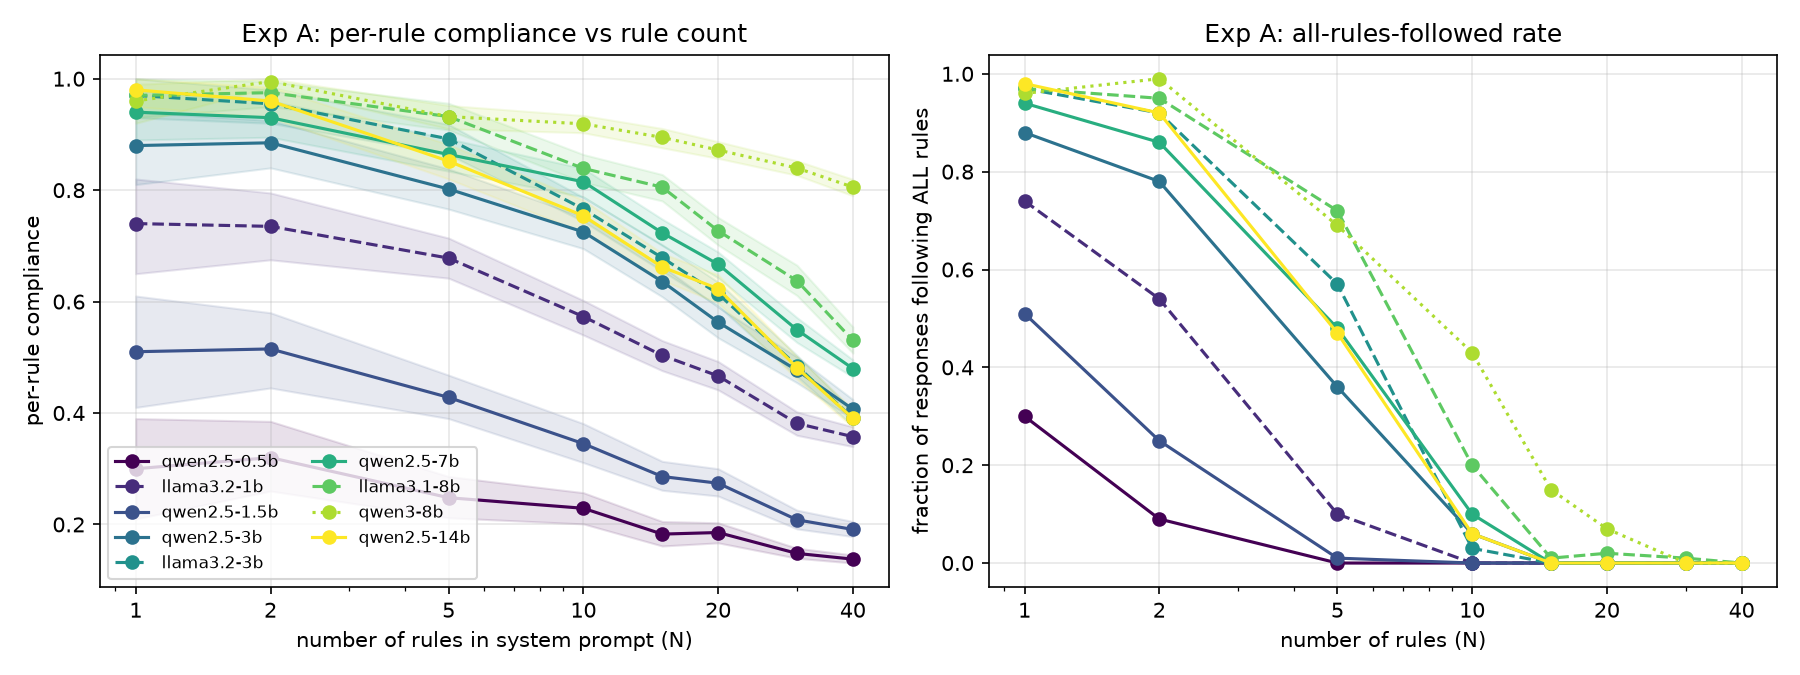
\includegraphics[width=0.95\linewidth]{figures/expA_count.png}
    \caption{\expA: rule count. \figleft Per-rule compliance with item-clustered 95\% bootstrap bands. Every model declines from about five rules onward, with no sharp knee. \qwenthree (dotted) stays near 0.8 even at 40 rules, while \qfourteen (yellow) tracks the 3B models. \figright The fraction of responses that follow {\em all} rules collapses to near zero by $N{=}15$ for every model except \qwenthree.}
    \label{fig:count}
\end{figure}

\begin{table}[t]
    \centering
    \caption{\expA: per-rule compliance (top) and chance-corrected retention $R(N)$ relative to $N{=}1$--2 (bottom). ``First $N$ $<$90\%'' is the smallest rule count at which retention falls below 0.9. Best value in each row in \textbf{bold}.}
    \label{tab:count}
    \resizebox{\textwidth}{!}{%
    \begin{tabular}{@{}lccccccccc@{}}
        \toprule
        & \multicolumn{5}{c}{\textbf{$<$7B}} & \multicolumn{4}{c}{\textbf{$\ge$7B}} \\
        \cmidrule(lr){2-6} \cmidrule(lr){7-10}
        & \textsc{Q-0.5B} & \textsc{L-1B} & \textsc{Q-1.5B} & \textsc{Q-3B} & \textsc{L-3B} & \textsc{Q-7B} & \textsc{L-8B} & \textsc{Qwen3-8B} & \textsc{Q-14B} \\
        \midrule
        \multicolumn{10}{@{}l}{\em Per-rule compliance} \\
        $N{=}1$  & .30 & .74 & .51 & .88 & .97 & .94 & .97 & .96 & \textbf{.98} \\
        $N{=}5$  & .25 & .68 & .43 & .80 & .89 & .86 & \textbf{.93} & \textbf{.93} & .85 \\
        $N{=}10$ & .23 & .57 & .35 & .73 & .77 & .82 & .84 & \textbf{.92} & .75 \\
        $N{=}20$ & .19 & .47 & .27 & .56 & .61 & .67 & .73 & \textbf{.87} & .62 \\
        $N{=}40$ & .14 & .36 & .19 & .41 & .39 & .48 & .53 & \textbf{.80} & .39 \\
        \midrule
        \multicolumn{10}{@{}l}{\em Chance-corrected retention $R(N)$} \\
        $N{=}10$ & .59 & .73 & .58 & .79 & .77 & .85 & .84 & \textbf{.93} & .74 \\
        $N{=}20$ & .36 & .56 & .39 & .58 & .59 & .67 & .72 & \textbf{.89} & .60 \\
        $N{=}40$ & .12 & .37 & .19 & .37 & .31 & .43 & .47 & \textbf{.80} & .31 \\
        First $N$ $<$90\% & 5 & 5 & 5 & 5 & 5 & 5 & 10 & \textbf{20} & 5 \\
        \bottomrule
    \end{tabular}}
\end{table}

{\bf Is there a saturation point?}
H4 predicts a knee: small models should hold steady up to about 10 rules and large models up to about 20.
\Figref{fig:count} and \tabref{tab:count} show no such knee.
Per-rule compliance starts to fall at $N{=}5$ for every model and keeps falling roughly log-linearly up to $N{=}40$.
Hinge regressions place the best breakpoint anywhere between 5 and 30 rules, with no consistent pattern across models.
Retention first drops below 90\% at $N{=}5$ for seven of nine models, at $N{=}10$ for \leight, and at $N{=}20$ for \qwenthree.

{\bf Does size help?}
Larger models degrade more slowly on average.
The 7--8B models keep 84--85\% of their chance-corrected single-rule compliance at 10 rules and 67--72\% at 20; the sub-3B models keep 58--73\% at 10 rules and 36--56\% at 20.
But size alone is a poor predictor.
\qfourteen retains only 74\% at 10 rules, below \qthree (79\%) and \qseven (85\%).
\qwenthree is in a class of its own, with 0.92 per-rule compliance at 10 rules and 0.80 at 40 rules, where the next-best model reaches 0.53.
Among models of similar size, the training recipe matters more than the parameter count.

{\bf Is this a length effect in disguise?}
In \expA, count and length grow together.
\expE holds length at about 4k tokens and still finds a decline with $N$ for all six models that ran it (\appref{app:expE}).
For example, from $N{=}5$ to $40$, \leight falls from 0.44 to 0.27 and \lthree from 0.44 to 0.24.
The slope is flatter than in \expA because 4k tokens of padding already push compliance toward the floor.

%-------------------------------------------------------------------
\subsection{Prompt length: a steep, early decline (H1)}
\label{sec:length}

\begin{figure}[t]
    \centering
    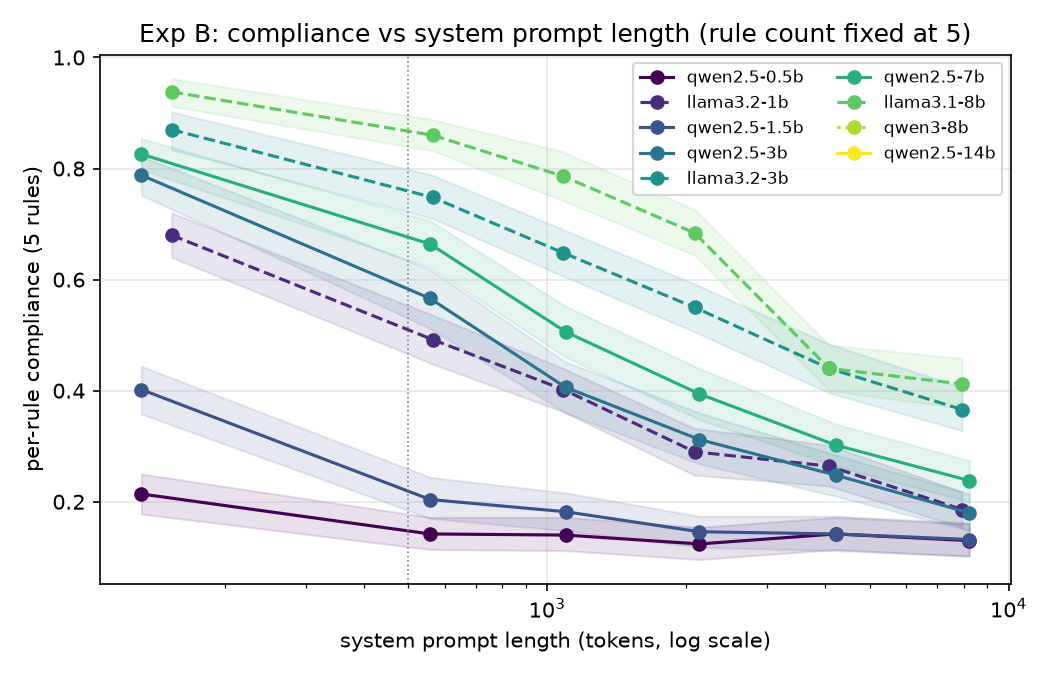
\includegraphics[width=0.62\linewidth]{figures/expB_length.png}
    \caption{\expB: per-rule compliance with five rules as a function of total system-prompt length (log scale; dotted line at 500 tokens). Bands are 95\% bootstrap CIs. Compliance falls steadily with every doubling, and the drop begins before 500 tokens. \qwenthree and \qfourteen did not complete \expB.}
    \label{fig:length}
\end{figure}

\begin{table}[t]
    \centering
    \caption{\expB: per-rule compliance with five interleaved rules as padding grows (left) and the slope per doubling of prompt length for prompts of at least 500 tokens (right; rule fixed effects, item-clustered 95\% CIs, Holm-corrected $p$). The pooled slope is about three to six times the hypothesized 2--5\% per doubling.}
    \label{tab:length}
    \resizebox{\textwidth}{!}{%
    \begin{tabular}{@{}lcccccccccc@{}}
        \toprule
        & \multicolumn{6}{c}{\textbf{Padding (tokens)}} & \multicolumn{3}{c}{\textbf{Slope per doubling}} \\
        \cmidrule(lr){2-7} \cmidrule(lr){8-10}
        \textbf{Model} & 0 & 500 & 1k & 2k & 4k & 8k & pp [95\% CI] & relative & Holm $p$ \\
        \midrule
        \qhalf    & .21 & .14 & .14 & .12 & .14 & .13 & $-$0.6 [$-$1.1, $-$0.1] & $-$4\% & 0.02 \\
        \lone     & .68 & .49 & .40 & .29 & .26 & .19 & $-$8.0 [$-$9.1, $-$6.9] & $-$16\% & $<$1e-30 \\
        \qonefive & .40 & .20 & .18 & .15 & .14 & .13 & $-$2.4 [$-$3.1, $-$1.6] & $-$12\% & $<$1e-9 \\
        \qthree   & .79 & .57 & .41 & .31 & .25 & .18 & $-$10.0 [$-$11.2, $-$8.8] & $-$18\% & $<$1e-50 \\
        \lthree   & .87 & .75 & .65 & .55 & \textbf{.44} & .37 & $-$9.7 [$-$10.9, $-$8.5] & $-$13\% & $<$1e-50 \\
        \qseven   & .83 & .66 & .51 & .39 & .30 & .24 & $-$11.0 [$-$12.0, $-$9.9] & $-$17\% & $<$1e-80 \\
        \leight   & \textbf{.94} & \textbf{.86} & \textbf{.79} & \textbf{.68} & \textbf{.44} & \textbf{.41} & $-$12.5 [$-$13.7, $-$11.4] & $-$15\% & $<$1e-90 \\
        \midrule
        Pooled (7 models) & & & & & & & $-$7.7 [$-$8.3, $-$7.1] & $-$15\% & 2e-149 \\
        \bottomrule
    \end{tabular}}
\end{table}

{\bf How fast does compliance fall with length?}
\Figref{fig:length} and \tabref{tab:length} show the result of holding the rule count at five and adding neutral padding.
Pooled over seven models, per-rule compliance falls by 7.7\pp per doubling beyond 500 tokens (95\% CI 7.1--8.3), about 15\% in relative terms.
H1 predicted 2--5\%, so the direction holds but the effect is three to six times larger.
For models that are competent at short lengths, the slope is 8--12.5\pp per doubling.
\qseven goes from 0.83 with no padding to 0.24 at about 8k tokens, and \qthree from 0.79 to 0.18.

{\bf When does the decline start?}
The decline begins well before 500 tokens.
Adding the first 500 tokens of padding costs 8--22\pp in competent models.
The two smallest Qwen models have small slopes only because they are already near their base rates without padding.

%-------------------------------------------------------------------
\subsection{Position: primacy in lists, recency in long prompts (H2)}
\label{sec:position}

\begin{figure}[t]
    \centering
    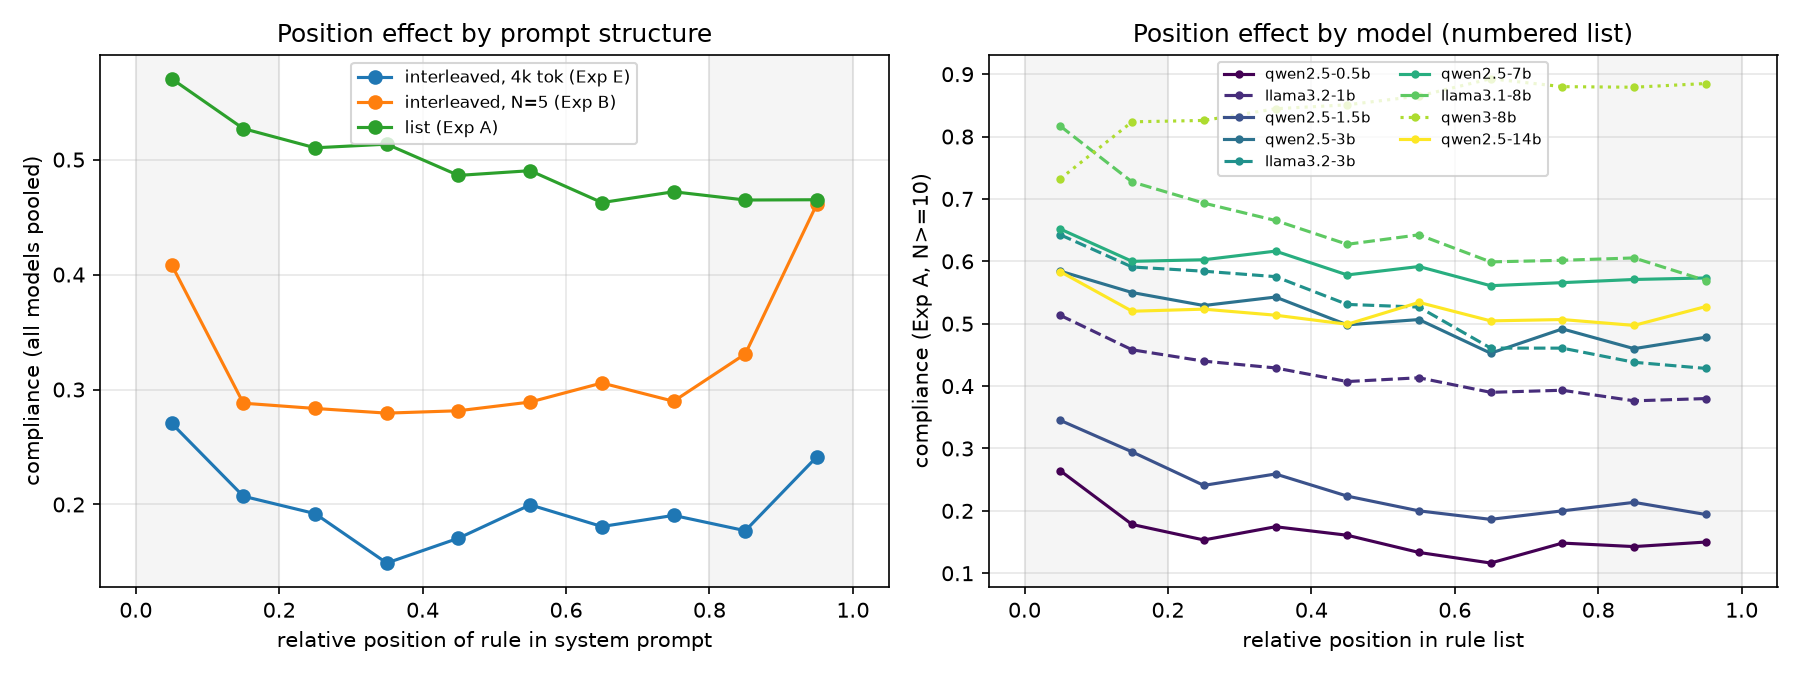
\includegraphics[width=0.95\linewidth]{figures/position.png}
    \caption{Compliance by relative rule position (deciles; shaded regions mark the first and last 20\%). \figleft Pooled over models. Rules in a short numbered list (\expA, green) show mild primacy and no end advantage. Rules interleaved in long padding (\expB, orange; \expE, blue) show a U-shape with the strongest effect at the end. \figright Per-model curves for numbered lists with $N \ge 10$. Most models favor early rules; \qwenthree (dotted) is the exception and favors late rules.}
    \label{fig:position}
\end{figure}

\begin{table}[t]
    \centering
    \caption{Compliance by rule position, pooled over models with rule and condition fixed effects. The ratio compares the mean of the two edge bins to the middle (95\% bootstrap CI). Differences are fixed-effect estimates; *** $p < 0.001$. H2 predicts a ratio of 1.15--1.25.}
    \label{tab:position}
    \resizebox{\textwidth}{!}{%
    \begin{tabular}{@{}lcccccc@{}}
        \toprule
        \textbf{Structure} & \textbf{First 20\%} & \textbf{Middle} & \textbf{Last 20\%} & \textbf{Edge / middle} & \textbf{First vs.\ mid} & \textbf{Last vs.\ mid} \\
        \midrule
        Numbered list (\expA, $N \ge 10$)          & \textbf{.550} & .489 & .465 & 1.04 [1.02, 1.06] & +5.0\pp*** & $-$2.8\pp*** \\
        Interleaved, $N{=}5$ (\expB, $\ge$1k tokens) & .365 & .287 & \textbf{.412} & \textbf{1.36} [1.23, 1.49] & +7.1\pp*** & +9.4\pp*** \\
        Interleaved, $\sim$4k tokens (\expE)       & \textbf{.239} & .180 & .212 & 1.25 [1.15, 1.35] & +6.0\pp*** & +4.9\pp*** \\
        \bottomrule
    \end{tabular}}
\end{table}

{\bf Are rules at the edges followed more often?}
The answer depends on how the rules are laid out (\tabref{tab:position}, \figref{fig:position}).
In a plain numbered list, the first 20\% of rules gain 5.0\pp (about 10\% relative) over the middle, but the last 20\% lose 2.8\pp.
The edge-to-middle ratio is only 1.04, far below the predicted 1.15--1.25.
When rules are scattered through long padding, both edges gain and the end gains most: the ratio is 1.36 for \expB and 1.25 for \expE, which meets or exceeds the prediction.

{\bf Do models agree?}
In numbered lists, 8 of 9 models favor early rules: the first 20\% gain 3 to 13\pp and the last 20\% lose 0 to 9\pp.
\leight shows the strongest primacy (+12.8\pp for the first 20\%, $-$5.2\pp for the last 20\%), and \lthree shows a similar pattern (+8.7\pp, $-$9.3\pp).
\qwenthree is the reverse: its first 20\% lose 8.7\pp and its last 20\% gain 2.1\pp.

%-------------------------------------------------------------------
\subsection{Block placement: the end of the prompt wins}
\label{sec:placement}

\begin{figure}[t]
    \centering
    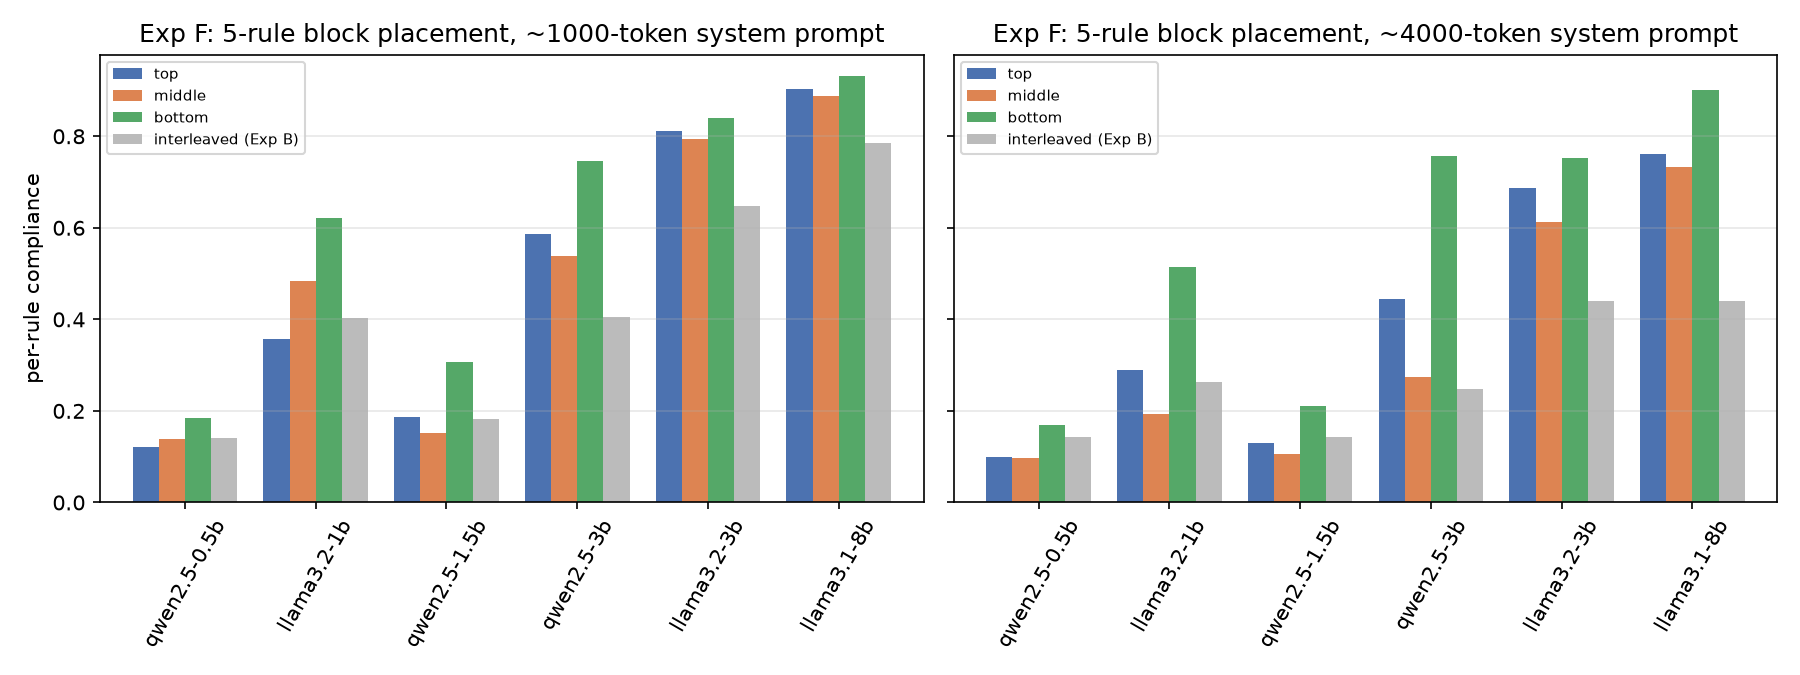
\includegraphics[width=0.95\linewidth]{figures/expF_placement.png}
    \caption{\expF: the same five rules as one numbered block placed at the top, middle, or bottom of a $\sim$1k-token \figleft or $\sim$4k-token \figright system prompt. Grey bars show the same rules interleaved through the padding (\expB). A block at the bottom, right before the user turn, is best for every model; at 4k tokens it recovers most of the loss for \qthree and \leight.}
    \label{fig:placement}
\end{figure}

\begin{table}[t]
    \centering
    \caption{\expF: per-rule compliance for a five-rule block at different positions, pooled over six models (left), and pooled placement effects relative to the middle with rule and model fixed effects (right; 95\% CIs). Best placement in \textbf{bold}.}
    \label{tab:placement}
    \small
    \begin{tabular}{@{}lccccccc@{}}
        \toprule
        & \multicolumn{4}{c}{\textbf{Compliance}} & \multicolumn{2}{c}{\textbf{Effect vs.\ middle}} \\
        \cmidrule(lr){2-5} \cmidrule(lr){6-7}
        \textbf{Length} & Interleaved & Top & Middle & Bottom & Top & Bottom \\
        \midrule
        $\sim$1k tokens & .43 & .49 & .50 & \textbf{.61} & +1.7\pp ($p{=}0.11$) & \textbf{+11.0\pp} [8.9, 13.1] \\
        $\sim$4k tokens & .28 & .40 & .34 & \textbf{.55} & +6.3\pp [4.1, 8.4] & \textbf{+20.8\pp} [18.6, 23.0] \\
        \bottomrule
    \end{tabular}
\end{table}

{\bf Why does length hurt?}
\expB mixes two possible causes: rules move farther from the end of the prompt, and rules are scattered among unrelated text.
\expF separates them by keeping the five rules together in one block and moving only the block (\figref{fig:placement}, \tabref{tab:placement}).
At about 4k tokens, the pooled compliance is 0.55 for a block at the bottom, 0.40 at the top, 0.34 in the middle, and 0.28 for the same rules interleaved.
A bottom block beats a middle block by 11.0\pp at 1k tokens and by 20.8\pp at 4k tokens.
Both causes therefore matter: distance from the end of the prompt is the larger factor, and a contiguous block beats scattered rules at every placement.

The effect is large for individual models.
\qthree reaches 0.76 with a bottom block at 4k tokens, close to its no-padding score of 0.80, compared with 0.27 in the middle and 0.25 when interleaved.
\leight reaches 0.90 at the bottom, 0.73 in the middle, and 0.76 at the top, but only 0.44 when its rules are interleaved.

These findings reconcile the two position patterns in \secref{sec:position}.
In a short list, every rule is close to the end of the prompt, so order within the list matters most and primacy appears.
In a long prompt, distance from the end dominates.

%-------------------------------------------------------------------
\subsection{Conflicting rules: large drops and compromises (H3)}
\label{sec:conflict}

\begin{figure}[t]
    \centering
    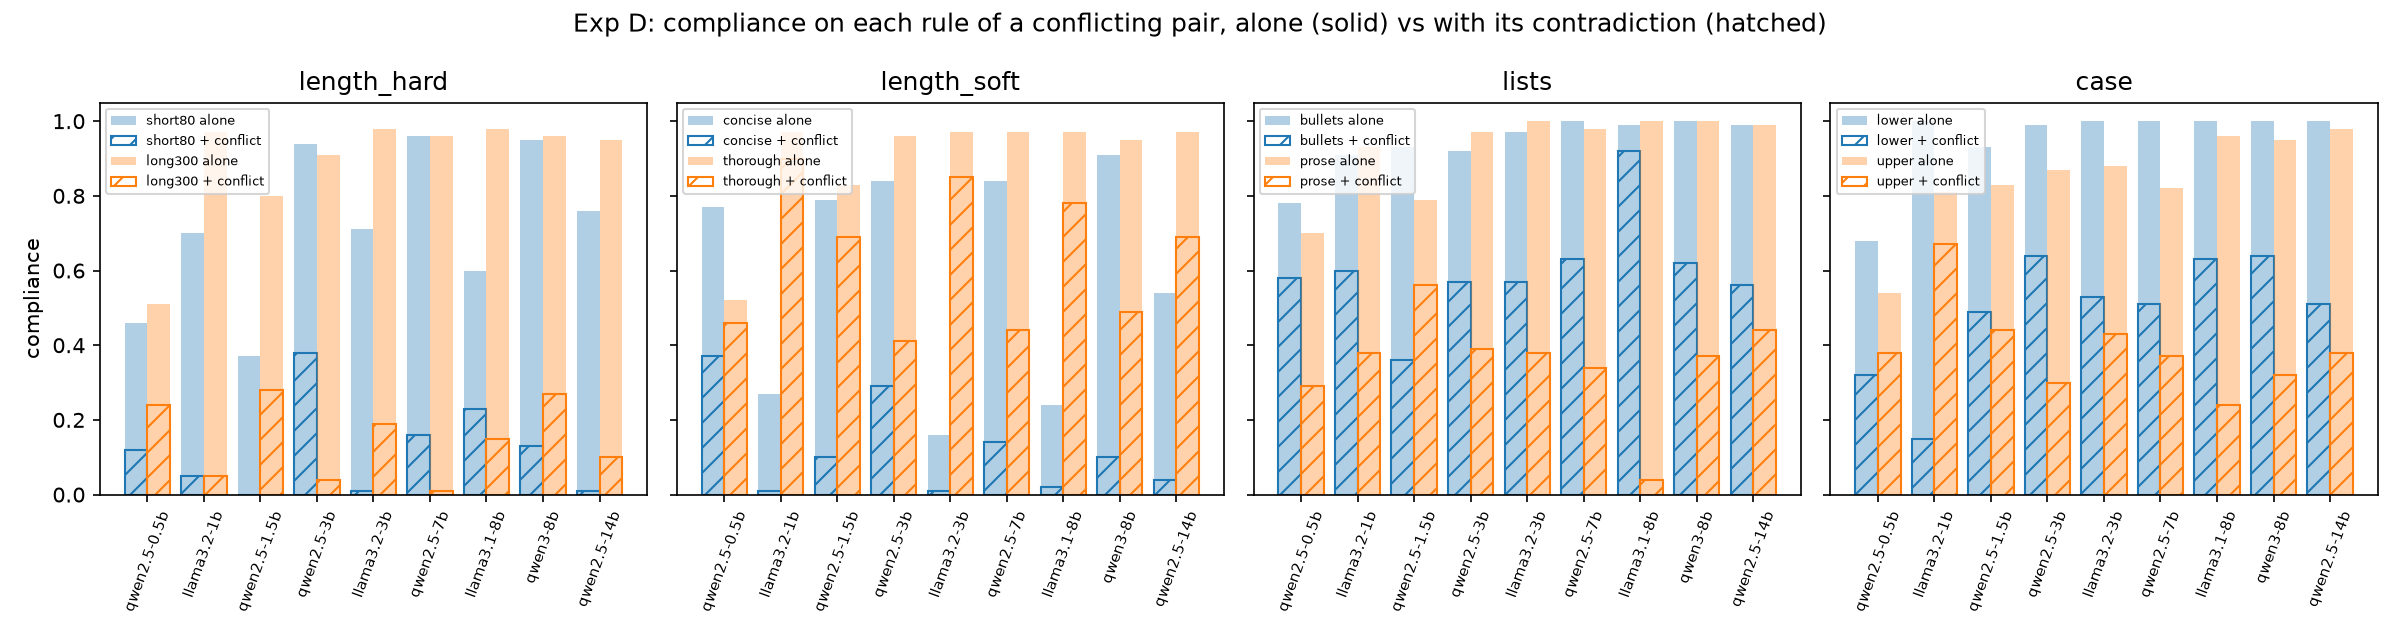
\includegraphics[width=\linewidth]{figures/expD_conflict.png}
    \caption{\expD: compliance with each rule of a contradictory pair when given alone (solid) and together with its contradiction (hatched), per model. For the length pairs, both hatched bars are often low at once, because responses settle on an intermediate length that satisfies neither rule. For \textsc{length\_soft}, the ``thorough'' rule (orange) keeps most of its compliance while ``concise'' collapses.}
    \label{fig:conflict}
\end{figure}

\begin{table}[t]
    \centering
    \caption{\expD: compliance on each member of a conflict pair, alone vs.\ with its contradiction, pooled over 9 models ($n{=}900$ paired items per row). Relative changes with 95\% bootstrap CIs. All rows have McNemar $p<10^{-10}$. The smallest drop is in \textbf{bold}; it is the only one inside the hypothesized 20--30\% band.}
    \label{tab:conflict}
    \small
    \begin{tabular}{@{}llccc@{}}
        \toprule
        \textbf{Pair} & \textbf{Rule} & \textbf{Alone} & \textbf{With contradiction} & \textbf{Relative change} \\
        \midrule
        \multirow{2}{*}{\textsc{length\_hard}} & $<$80 words & .72 & .12 & $-$83\% [$-$87, $-$79] \\
        & $\ge$300 words & .89 & .15 & $-$83\% [$-$87, $-$80] \\
        \midrule
        \multirow{2}{*}{\textsc{length\_soft}} & be concise ($<$150 w) & .60 & .12 & $-$80\% [$-$84, $-$75] \\
        & explain thoroughly ($\ge$250 w) & .90 & .63 & \textbf{$-$30\%} [$-$35, $-$25] \\
        \midrule
        \multirow{2}{*}{\textsc{lists}} & bulleted list & .94 & .60 & $-$36\% [$-$43, $-$29] \\
        & no lists & .93 & .35 & $-$62\% [$-$68, $-$55] \\
        \midrule
        \multirow{2}{*}{\textsc{case}} & all lowercase & .96 & .49 & $-$49\% [$-$53, $-$44] \\
        & ALL UPPERCASE & .85 & .39 & $-$54\% [$-$58, $-$49] \\
        \bottomrule
    \end{tabular}
\end{table}

{\bf How much does a contradiction cost?}
Adding the contradicting rule lowers compliance on each member of a pair by 30--83\% relative (\tabref{tab:conflict}).
Every pooled comparison has $p < 10^{-10}$, and 66 of the 72 per-model tests stay significant after Holm correction.
H3 predicted 20--30\%, so the direction holds but the drop is 1.5--3 times larger.
Because the rules in each pair are mutually exclusive, a large drop is expected; the more informative question is how models resolve the conflict.

{\bf How do models resolve conflicts?}
For length conflicts, models usually compromise and satisfy neither rule.
With ``fewer than 80 words'' plus ``at least 300 words'', 58\% (\qthree) to 90\% (\lone) of responses meet neither constraint.
The median length with both rules is 96--220 words, compared with about 50--90 words for the short rule alone and about 350--500 words for the long rule alone.
For format and case conflicts, one rule usually wins: ``neither'' outcomes are only 0--13\% for 8 of 9 models.
The winner is stable within a model (\eg \leight chooses bullets 92\% of the time), and it is not simply the rule that appears later, since rule order was randomized.

{\bf Is the soft conflict symmetric?}
No.
Every model leans toward ``explain thoroughly'': ``be concise'' loses 80\% of its compliance, while ``explain thoroughly'' loses only 30\%.
This is the only result inside the hypothesized 20--30\% band.

{\bf Do conflicts hurt other rules?}
Barely.
Background keyword rules move by only 0--8\pp between conflict and no-conflict conditions, with no consistent sign.
The cost of a contradiction stays within the contradicting pair.

%-------------------------------------------------------------------
\subsection{Qualitative analysis and reproducibility}
\label{sec:qualitative}

\para{Rules are silently dropped.}
At 8k tokens, \qseven writes well-formed, on-topic answers that ignore most rules.
It is not confused by the padding; it behaves as if the rules were not there.
Rules that responses often satisfy naturally survive (bold text, numbered lists, exclusions), while arbitrary keywords such as ``velvet'', ``pineapple'', ``consequently'', and ``indeed'' twice fall to nearly zero at 4--8k tokens.

\para{Compromises can be strange.}
Given ``fewer than 80 words'' and ``at least 300 words'', \qseven wrote 143 words.
Given ``all lowercase'' and ``all UPPERCASE'' together with a rule to include ``gracias'', it wrote its name ``orion'' in lowercase and then switched to an all-caps answer in Spanish.
Satisfying one rule spilled over into an odd reading of another.

\para{Exclusion rules carry little signal.}
Rules such as ``never use {\em really}'' have base rates of 81--99\%, so they look followed regardless of condition.
The headline effects come from inclusion and format rules, and the retention metric corrects for this.

\para{Reproducibility.}
We re-ran \qonefive on all of \expA (900 prompts, 12{,}300 rule checks) in a separate process on a different GPU with a different KV-cache size.
Because vLLM greedy decoding is not batch-invariant, only 13\% of responses were byte-identical.
Even so, 93.7\% of individual rule checks agreed, and mean compliance changed by only 0.07\pp (0.2503 vs.\ 0.2496).
Aggregate effects are therefore stable under decoding noise, even though single responses are not deterministic.

\section{Discussion}
\label{sec:discussion}

\para{Dilution, not saturation.}
H4 pictures rule-following as a capacity that fills up: a model handles rules perfectly until it runs out of room.
Our data do not show this.
Every model loses compliance from about the fifth rule onward, and the curve is smooth rather than a cliff.
A better description is dilution: each additional rule, and each additional thousand tokens between a rule and the user turn, lowers the chance that any given rule shapes the output.
Model quality sets both the starting level and the rate of decline, but no tested model stays flat to 20 rules.
\qwenthree comes closest (0.92 at 10 rules, 0.87 at 20), which suggests that newer instruction-tuning recipes matter more than raw scale.
\qfourteen did not beat \qseven; this could be partly due to quantization, but it fits the view that scale alone does not buy rule capacity.

\para{Length hurts through distance and burial.}
Comparing \expB and \expF, the same five rules in a 4k-token prompt are followed 28\% of the time when scattered, 34\% as a block in the middle, 40\% as a block at the top, and 55\% as a block at the bottom.
Chat models appear to weight the most recent system text heavily when they decide on format and content.
For short lists, the first rules benefit instead.
The two patterns are consistent once we note that in a short list all rules are already close to the end.

\para{Contradictions are costly.}
Contradictory rules do more than force a choice.
For numeric constraints, models often split the difference and fail both rules, so a contradictory pair can be worse than dropping one of its rules.
For soft conflicts, the ``thorough'' instruction reliably wins.

\para{Practical guidance.}
Our results suggest three rules of thumb for prompt authors.
First, every rule has a cost, starting with the first few, so prompts should contain only rules that matter.
Second, in long system prompts, critical rules should sit in one contiguous block at the end, right before the user turn; in short rule lists, the most important rules should come first.
Third, prompts should be checked for contradictions, because models seldom resolve them gracefully.

\subsection{Limitations}
\label{sec:limitations}

\para{Open models only.}
No API keys were available, so we could not test commercial frontier models.
These may be much more robust; \qwenthree already is.

\para{Quantization is confounded with size.}
The 3B, 8B, and 14B models are AWQ int4, while the 0.5B--1.5B and 7B models are bf16.
The finding that \qfourteen does not beat \qseven may partly reflect quantization.

\para{Incomplete coverage.}
Shared-GPU contention meant that \expB covers 7 models, \expE and \expF cover 6, and \qwenthree and \qfourteen have only \expA and \expD.
Our length and placement conclusions therefore do not include the two strongest models on the count experiment.

\para{Synthetic rules and padding.}
Our rules are verifiable but artificial: arbitrary keywords and formats.
Real system-prompt rules (tone, refusals, tool policies) may behave differently.
Inclusion rules are harder than natural ones, and exclusion rules sit near ceiling.
Our padding is encyclopedic text labeled as background; realistic padding such as tool documentation may compete with rules more or less strongly.

\para{Design confounds and variance.}
In \expA, count and length grow together; \expE addresses this only for the models that ran it.
Each model was run once with greedy decoding, and run-to-run variance from batch non-invariance was checked on one model only.
Our confidence intervals cover query sampling, not decoding noise.
Finally, we test only single-turn answers of about 100--500 words.

\para{Broader impact.}
System-prompt rules often encode safety and policy constraints.
Our results show that such rules can be silently dropped in long prompts, so deployers should not assume that a rule written into a system prompt will be enforced.
Measuring rule compliance under realistic prompt lengths should be part of deployment testing.

\section{Conclusion}
\label{sec:conclusion}

We tested four quantitative claims about system-prompt compliance with a controlled benchmark of 40 verifiable rules and 4 conflict pairs on 9 open models.
Compliance degrades continuously.
It falls by about 7.7\pp (15\% relative) per doubling of prompt length at a fixed rule count, declines with every rule added from about five rules on, and drops by 30--83\% when rules contradict.
All of these effects are steeper than the hypothesized magnitudes, and the predicted size thresholds of 10 and 20 rules did not appear.
Model recipe mattered more than parameter count.

The key takeaway is about placement: in long system prompts, put the rules that must be followed in one block at the end; in short rule lists, put the most important rules first.

Several directions follow.
We plan to repeat the study with frontier API models and with bf16 versions of the 3B, 8B, and 14B models; to use realistic rule types such as tone, refusal, and tool-use policies, scored by an LLM judge; to fully cross placement, count, and length, including repeating critical rules at the end; to study multi-turn sessions; and to test whether explicit priority markers or a stated conflict-resolution order prevent compromises that satisfy neither rule.


\bibliography{references}

\appendix
\section{Rule Count at a Fixed Long Length (\expE)}
\label{app:expE}

\begin{figure}[h]
    \centering
    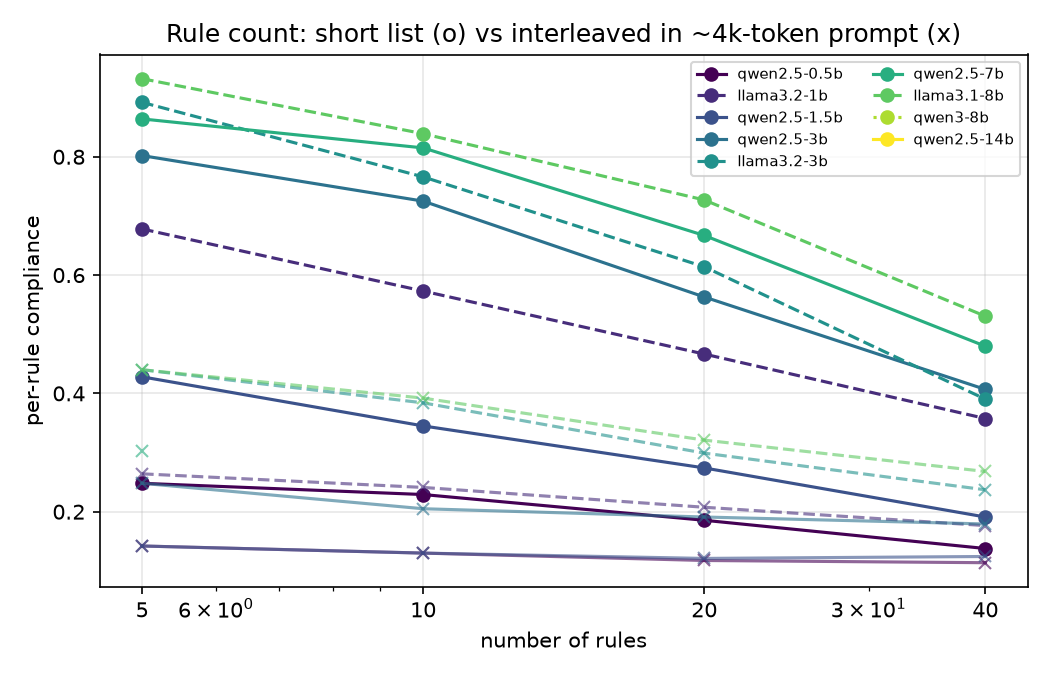
\includegraphics[width=0.62\linewidth]{figures/expE_count_long.png}
    \caption{\expE: per-rule compliance as the number of rules grows, with all rules interleaved in about 4k tokens of padding, compared with the short numbered-list format of \expA. Compliance still declines with rule count when length is held fixed, but from a much lower starting point.}
    \label{fig:expE}
\end{figure}

\begin{table}[h]
    \centering
    \caption{Per-rule compliance by rule count in a short numbered list (\expA) and interleaved in $\sim$4k tokens of padding (\expE; the $N{=}5$ column is from \expB at 4k tokens). \qseven did not run \expE.}
    \label{tab:expE}
    \small
    \begin{tabular}{@{}lcccccccc@{}}
        \toprule
        & \multicolumn{4}{c}{\textbf{Short list (\expA)}} & \multicolumn{4}{c}{\textbf{Interleaved, $\sim$4k tokens}} \\
        \cmidrule(lr){2-5} \cmidrule(lr){6-9}
        \textbf{Model} & 5 & 10 & 20 & 40 & 5 & 10 & 20 & 40 \\
        \midrule
        \qhalf    & .25 & .23 & .19 & .14 & .14 & .13 & .12 & .11 \\
        \lone     & .68 & .57 & .47 & .36 & .26 & .24 & .21 & .18 \\
        \qonefive & .43 & .35 & .27 & .19 & .14 & .13 & .12 & .12 \\
        \qthree   & .80 & .73 & .56 & .41 & .25 & .21 & .19 & .18 \\
        \lthree   & .89 & .77 & .61 & .39 & \textbf{.44} & .38 & .30 & .24 \\
        \leight   & \textbf{.93} & \textbf{.84} & \textbf{.73} & \textbf{.53} & \textbf{.44} & \textbf{.39} & \textbf{.32} & \textbf{.27} \\
        \bottomrule
    \end{tabular}
\end{table}

\section{Conflict Resolution Details}
\label{app:conflict}

\begin{table}[h]
    \centering
    \caption{\expD: share of responses that satisfy only rule X, only rule Y, or neither, when both contradictory rules are present (``both'' is impossible). X is the first-listed rule of each pair: $<$80 words, concise, bulleted list, lowercase. Largest share per model and pair in \textbf{bold}.}
    \label{tab:winner}
    \resizebox{\textwidth}{!}{%
    \begin{tabular}{@{}lcccccccccccc@{}}
        \toprule
        & \multicolumn{3}{c}{\textsc{length\_hard}} & \multicolumn{3}{c}{\textsc{length\_soft}} & \multicolumn{3}{c}{\textsc{lists}} & \multicolumn{3}{c}{\textsc{case}} \\
        \cmidrule(lr){2-4} \cmidrule(lr){5-7} \cmidrule(lr){8-10} \cmidrule(lr){11-13}
        \textbf{Model} & X & Y & neither & X & Y & neither & X & Y & neither & X & Y & neither \\
        \midrule
        \qhalf     & .12 & .24 & \textbf{.64} & .37 & \textbf{.46} & .17 & \textbf{.58} & .29 & .13 & .32 & \textbf{.38} & .30 \\
        \lone      & .05 & .05 & \textbf{.90} & .01 & \textbf{.90} & .09 & \textbf{.60} & .38 & .02 & .15 & \textbf{.67} & .18 \\
        \qonefive  & .00 & .28 & \textbf{.72} & .10 & \textbf{.69} & .21 & .36 & \textbf{.56} & .08 & \textbf{.49} & .44 & .07 \\
        \qthree    & .38 & .04 & \textbf{.58} & .29 & \textbf{.41} & .30 & \textbf{.57} & .39 & .04 & \textbf{.64} & .30 & .06 \\
        \lthree    & .01 & .19 & \textbf{.80} & .01 & \textbf{.85} & .14 & \textbf{.57} & .38 & .05 & \textbf{.53} & .43 & .04 \\
        \qseven    & .16 & .01 & \textbf{.83} & .14 & \textbf{.44} & .42 & \textbf{.63} & .34 & .03 & \textbf{.51} & .37 & .12 \\
        \leight    & .23 & .15 & \textbf{.62} & .02 & \textbf{.78} & .20 & \textbf{.92} & .04 & .04 & \textbf{.63} & .24 & .13 \\
        \qwenthree & .13 & .27 & \textbf{.60} & .10 & \textbf{.49} & .41 & \textbf{.62} & .37 & .01 & \textbf{.64} & .32 & .04 \\
        \qfourteen & .01 & .10 & \textbf{.89} & .04 & \textbf{.69} & .27 & \textbf{.56} & .44 & .00 & \textbf{.51} & .38 & .11 \\
        \bottomrule
    \end{tabular}}
\end{table}

\begin{table}[h]
    \centering
    \caption{\expD: median response length (words) for the length pairs with only rule X, only rule Y, or both rules, and with no rules ($N{=}0$). With both rules, responses settle between the two targets.}
    \label{tab:wordcounts}
    \small
    \begin{tabular}{@{}lccccccc@{}}
        \toprule
        & \multicolumn{3}{c}{\textsc{length\_hard}} & \multicolumn{3}{c}{\textsc{length\_soft}} & \\
        \cmidrule(lr){2-4} \cmidrule(lr){5-7}
        \textbf{Model} & $<$80 & both & $\ge$300 & concise & both & thorough & no rules \\
        \midrule
        \qhalf     & 81.5 & 138.0 & 300.5 & 83.0 & 227.0 & 260.0 & 193.5 \\
        \lone      & 74.0 & 153.0 & 472.5 & 192.0 & 336.0 & 487.5 & 375.5 \\
        \qonefive  & 90.5 & 204.5 & 399.0 & 103.0 & 291.0 & 361.0 & 191.5 \\
        \qthree    & 46.0 & 96.0 & 423.5 & 95.5 & 200.0 & 434.5 & 333.0 \\
        \lthree    & 74.0 & 219.5 & 453.5 & 199.5 & 319.5 & 427.0 & 321.5 \\
        \qseven    & 51.0 & 103.0 & 456.0 & 103.0 & 234.0 & 436.0 & 312.0 \\
        \leight    & 76.0 & 102.0 & 496.0 & 183.0 & 320.5 & 473.0 & 350.5 \\
        \qwenthree & 56.0 & 158.0 & 354.0 & 87.5 & 241.5 & 437.5 & 392.0 \\
        \qfourteen & 67.5 & 164.0 & 434.5 & 139.5 & 295.0 & 401.5 & 342.0 \\
        \bottomrule
    \end{tabular}
\end{table}

\section{Prompt Templates}
\label{app:templates}

In \expA, the system prompt reads ``You are a helpful assistant. Follow these rules in every response:'' followed by the rules as a numbered list.
In \expB and \expE, the prompt opens with: ``You are a helpful assistant. The reference material below is provided for background only. Rules for your responses are marked `Response rule:' and appear throughout this prompt; follow all of them.''
Each rule is then inserted as a standalone paragraph beginning with ``Response rule:'' at a random paragraph boundary of the padding, which is introduced as ``Reference material (background only):''.
In \expF, the five rules form one numbered block placed before, inside, or after the padding.
All prompts are built with seed 42; rule subsets, rule order, and padding paragraphs are drawn independently for each item.


\end{document}
